\documentclass [a4paper,12pt,openany,italian,oneside]{book}
\usepackage[italian]{babel}
\usepackage[T1]{fontenc}
\usepackage[utf8x]{inputenc}
\usepackage{lmodern}
\usepackage{graphicx}
\usepackage{amssymb}
\usepackage{enumitem}
\usepackage{indentfirst}
\usepackage[font={small,it},labelfont=bf]{caption}
\usepackage{verbatim}
\usepackage{natbib}
\usepackage[nottoc,notlot,notlof]{tocbibind}
\usepackage[plainpages=false]{hyperref}
\usepackage{amsmath}
\usepackage[chapter]{algorithm}
\usepackage[noend]{algpseudocode}
\usepackage{booktabs}

\floatname{algorithm}{Algoritmo}

\usepackage{xargs}
\usepackage[colorinlistoftodos,prependcaption,textsize=tiny]{todonotes}
\newcommandx{\unsure}[2][1=]{\todo[linecolor=red,backgroundcolor=red!25,bordercolor=red,#1]{#2}}
\newcommandx{\change}[2][1=]{\todo[linecolor=blue,backgroundcolor=blue!25,bordercolor=blue,#1]{#2}}
\newcommandx{\info}[2][1=]{\todo[linecolor=OliveGreen,backgroundcolor=OliveGreen!25,bordercolor=OliveGreen,#1]{#2}}
\newcommandx{\improvement}[2][1=]{\todo[linecolor=violet,backgroundcolor=violet!25,bordercolor=violet,#1]{#2}}

\bibliographystyle{plain}
\setcounter{tocdepth}{1}
\setcounter{secnumdepth}{3}

\newlist{Properties}{enumerate}{1}
\setlist[Properties]{label=\textbf{Proprietà \arabic*.},itemindent=* }
\algnewcommand{\LeftComment}[1]{\Statex \(\triangleright\) #1}

\makeatletter
\def\BState{\State\hskip-\ALG@thistlm}
\makeatother

\begin{document}

%parte iniziale
\frontmatter
\pagestyle{plain}
\thispagestyle{empty}
\begin{center}
	\vspace{10mm}
	{
\includegraphics[width=0.4 \linewidth]{img/uniroma3-logo}} \\
	\vspace{10mm}
	{\Large UNIVERSIT\`A DEGLI STUDI ROMA TRE} \\
	\vspace{5mm}
	{\Large Facolt\`a di Ingegneria} \\
	{\Large Corso di Laurea Magistrale in Ingegneria Informatica} \\
	\vspace{15mm}
	{\Large Tesi di Laurea Magistrale} \\
	\vspace{10mm}
	{\Large \textbf{Progettazione di una blockchain scalabile senza impatto su decentralizzazione e sicurezza}} \\
	\vspace{4 cm}
	\noindent \textbf{Relatore} \hfill \textbf{Laureando} \\
	\noindent Prof. Maurizio Pizzonia \hfill Gianmaria Del Monte \\
	\hfill 499829 \\
	\noindent  \textbf{Correlatore} \hfill {.}\\
	\noindent Diego Pennino \hfill {.}\\
	\vfill
	{\large Anno Accademico 2019/2020} \\
\end{center}
\newpage
\thispagestyle{empty}
\null\vspace{\stretch{1}}
\begin{flushright}
\emph{{a Clara,\\a Silvia,\\ai miei genitori}}
\end{flushright}
\vspace{\stretch{2}}\null
\newpage
\listoftodos
\chapter{Introduzione}

Le blockchain permettono di creare applicazioni che offrono integrità dei dati, trasparenza e immutabilità, senza alcuna autorità centrale che regoli le transazioni. La decentralizzazione ha aperto nuove strade in molti campi, ad esempio quello finanziario, ma pone delle nuove sfide per assicurare la consistenza su tutti i nodi della rete. Una blockchain pubblica per essere adottata a livello globale deve essere decentralizzata, sicura e scalabile. I tre requisiti, certamente contrastanti, determinano una difficoltà in fase di progettazione di una blockchain che li contempli tutti e tre. Vitalik Buterin, fondatore di Ethereum, ha espresso questa difficoltà nel celebre \textit{blockchain scalability trilemma}. Secondo il trilemma una blockchain può massimizzare solo due delle tre proprietà a scapito della terza.

Negli attuali sistemi di blockchain, ogni nodo riceve e processa tutte le transazioni generate nella rete. Questo è quindi un problema per la scalabilità, poiché ogni nodo rappresenta un collo di bottiglia per la sua banda e potenza computazionale limitata. In letteratura sono stati proposti sia approcci focalizzati sulla scalabilità del consenso, come Algorand~\cite{gilad2017algorand}, sia da un punto di vista architetturale, mediante lo \textit{sharding} (adottato anche nei sistemi di database distribuiti). Lo sharding consiste nel partizionare l'intera rete in tante sottoreti di piccole dimensioni, denominate \textit{shard}, in cui ognuna è responsabile di un sottoinsieme dello stato memorizzato in blockchain. Benché sia una soluzione alla scalabilità, lo sharding penalizza la sicurezza, poiché gli shard sono composti da pochi nodi rispetto a quelli presenti sulla tutta la rete. Inoltre, rende difficile la gestione di transazioni \textit{cross-shard}.

In questo lavoro di tesi, si introduce da un punto di vista teorico un'architettura in grado di scalare proporzionalmente il numero dei nodi con il throughput delle transazioni. La soluzione è architetturale e tiene conto di tutti i suoi aspetti (consenso, comunicazione e storage). In questa nuova proposta, nessun nodo invia in broadcast le transazioni che genera e non è obbligato a ricevere e processare tutte le transazioni create in un round. La scalabilità in questo caso non ha impatto né su decentralizzazione, né sulla sicurezza. Infatti, ogni nodo contribuisce alla conferma delle transazioni con un ruolo scelto in modo efficiente mediante una selezione randomica, basata sulle \textit{Verifiable Random Function}. Inoltre, l'incremento del throughput delle transazioni non necessita di una diminuzione del numero di nodi aventi lo stesso ruolo, come avviene in approcci sharded. Il contributo di questa tesi dimostra da un punto di vista formale che è possibile risolvere il blockchain scalability trilemma.

La presente tesi è suddivisa in tre capitoli. Il primo capitolo presenta un'introduzione al tema delle blockchain, presentando la sua prima realizzazione, ovvero Bitcoin, per poi passare alle strutture dati autenticate e alle Distributed Hash Table, che saranno utili per la definizione dell'architettura proposta. Il secondo capitolo è dedicato allo stato dell'arte, presentando Algorand~\cite{gilad2017algorand}, una soluzione ai problemi di scalabilità degli algoritmi di consenso in approcci basati su Bitcoin, ponendo attenzione ad un approccio strutturale~\cite{bernardini2019blockchains} che consente ai nodi della rete di non dover memorizzare l'intero stato della blockchain, pur rimanendo in grado di validare le nuove transazione ed infine un analisi sulle architetture basate sullo sharding. Nel terzo capitolo sono analizzate le problematiche delle soluzioni correnti ed è presentata la nuova architettura proposta con questo lavoro di tesi, con i relativi teoremi di correttezza e scalabilità.

\tableofcontents

%inizio capitoli
\mainmatter
\pagestyle{headings}
\chapter{Background}

\section{Bitcoin e Blockchain}
Bitcoin è una tecnologia open-source per lo scambio di valute, denominate \emph{bitcoin}, decentralizzato, presentato nel 2008 da una persona anonima, con lo pseudonimo di Satoshi Nakamoto \cite{nakamoto2019bitcoin}.
A differenza di valute tradizionali che esistono fisicamente sotto forma di banconote, i bitcoin sono monete virtuali. Esse vengono scambiate tra i partecipanti alla rete Bitcoin che comunicano mediante il protocollo Bitcoin. Quindi con il termine Bitcoin, si indicano vari aspetti: la tecnologia in sé, lo stack protocollare di comunicazione adottato tra i partecipanti alla rete e la valuta scambiata.
Bitcoin è una rete P2P, a cui partecipano nodi chiamati \emph{peer}, in cui non esistono nodi speciali o più importanti di altri, come nei sistemi di pagamento elettronici tradizionali, in cui c'è un server centrale che gestisce tutti i pagamenti.

Il concetto fondamentale di Bitcoin è quello di \emph{transazione}: una transazione trasferisce dei bitcoin da una conto sorgente ad un conto destinazione. Le transazioni possono sono create da qualsiasi peer della rete, che dimostri essere proprietario del conto sorgente e vengono inviate a tutti i nodi della rete. A differenza di pagamenti elettronici tradizionali, in cui un server centrale accetta o rifiuta le transazioni generate dai propri clienti, le transazioni sono accettate o rifiutate dalla rete Bitcoin secondo un meccanismo di \emph{consenso distribuito}, utilizzando un approccio denominato \emph{Proof-of-work}. La transazioni accettate vengono quindi raggruppate in blocchi di transazioni, secondo un processo che richiede un enorme quantità di potenza computazionale, che vengono aggiunti ai blocchi della \emph{blockchain}. Questo processo è definito \emph{mining} ed è svolto dai peer che ricoprono il ruolo di \emph{miners}. Il mining ha due obiettivi:
\begin{enumerate}
	\item creazione di bitcoin: ogni nodo che aggiunge un blocco alla blockchain viene ricompensato dalla rete con una quantità di bitcoin fissata per ogni blocco e che decresce nel tempo;
	\item validazione delle transazioni secondo le regole di consenso, assicurando che le transazioni siano non valide e non corrette.
\end{enumerate}
Inizialmente il mining veniva effettuato da personal computer potenti. Man mano che i miner si aggiungevano alla rete Bitcoin, per cui diveniva sempre più difficile \emph{minare} un blocco, si utilizzarono delle Graphical Processing Units, o GPU, come quelle utilizzate nei videogiochi. Tuttavia negli ultimi anni, a causa dell'elevato numero di miner presenti sulla rete, si utilizzano sistemi Application Specific Integrated Circuit, o ASIC, che implementano in hardware gli algoritmi di mining impiegati in Bitcoin per aumentare le performance. Sono state create anche soluzioni che hanno l'obiettivo di condividere la propria potenza computazionale in mining farm, o mining pool, con diversi partecipanti, in cui si suddividono i bitcoin guadagnati.

\subsection{Wallet e indirizzi digitali}
Un nodo per partecipare alla rete e scambiare i propri bitcoin, ha bisogno di una \emph{chiave digitale} e di un \emph{bitcoin address}. Un utente può generare un numero qualsiasi di chiavi digitali, che vengono memorizzate in un database locale, denominato \emph{wallet}.
La possibilità di generate autonomamente delle chiavi evidenza la caratteristica fondamentale di Bitcoin, ovvero quella della decentralizzazione del controllo e del consenso, basate su prove crittografiche.
In particolare, il modello di riferimento è quello della crittografia a chiave asimmetrica, in cui le chiavi digitali sono sottoforma di una coppia di chiavi, una \emph{privata}, segreta, ed una \emph{pubblica}, che deriva dalla chiave privata. \'E importante specificare che l'uso della crittografia non ha uno scopo di \emph{confidenzialità}, d'altronde tutto in Bitcoin viaggia in chiaro, ma per \emph{autenticità}, per dimostrare quindi chi si dice di essere, ovvero possessori di un certo conto.
Secondo una relazione matematica, la chiave privata può essere usata per firmare un messaggio, o in questo caso una transazione,  e la chiave pubblica, conosciuta da tutti i nodi della rete, per validare la firma del messaggio. Infatti, semplicisticamente, la chiave pubblica è usata per ricevere i bitcoin, mentre la chiave privata per spenderli, secondo delle modalità che saranno note nel proseguimento della lettura dei prossimi paragrafi, in cui si mostra la creazione di una transazione da parte di un client, e quindi le prove crittografiche che deve mostrare in modo da poter spendere i suoi bitcoin.
In una transazione, l'indirizzo di destinazione è indicato da un \emph{bitcoin address}, che deriva dalla chiave privata del client, mediante una serie di funzioni hash, come illustrato nella Figura~\ref{img:bit_address}.\todo{inserire immagine di come un indirizzo bitcoin deriva da una chiave pubblica}
Quando un nodo spende i propri bitcoin, associati al bitcoin address del nodo stesso, presenta la sua chiave pubblica e la firma di una certa stringa che dimostra che effettivamente lui è il proprietario di quella somma. In questo modo, chiunque nella rete, con queste due informazioni, può verificare che il nodo è realmente il proprietario di una certa quantità di bitcoin spesi in una transazione. \'E chiaro che chiunque in possesso della chiave privata di un nodo, può spendere a suo piacimento i bitcoin associati al relativo bitcoin address. Per questo, e anche per anonimizzare i creatori delle transazioni, un wallet genera ad ogni transazione una nuova coppia di chiavi.

Un waller, come si già è detto in precedenza, è un client che memorizza le chiavi digitali di un nodo. Può essere: (1) \emph{non-deterministico} e generare chiavi private in modo totalmente randomico, per cui il waller è un database che memorizza queste chiavi private, e (2) \emph{deterministico} e generare delle chiavi private a partire da un unico \emph{seed}, che può essere anche una password digitata da un utente, per cui non ha bisogno di memorizzare alcuna chiave.


\subsection{Transazioni}

Le transazioni ricoprono un ruolo fondamentale in Bitcoin e nelle tecnologie di blockchain in generale. Le transazioni sono delle strutture dati che codificano un trasferimento di bitcoin da una o più sorgenti, denominate \emph{input}, ad una o più destinazioni, denominate \emph{output}. I campi di una transazione sono riportati nella Tabella~\ref{tab:tx_fields}.
\change{cambiare stile tabella}

Vediamo ora il ciclo di vita di una transazione. Ogni nodo nella rete può generare una transazione. Il nodo durante la creazione può essere online o offline. La transazione contiene una firma che dimostra che il nodo possiede i bitcoin specificati nell'input. La transazione viene quindi inviata in broadcast, raggiungendo tutti i nodi della rete. Questa viene messa nella lista delle transazioni in attesa, \emph{pending transactions}, verificata da ogni nodo, e se è valida, ovvero è conforme alle regole di consenso, viene inclusa all'interno di un blocco insieme ad altre transazioni e aggiunta in coda alla blockchain.

\begin{table}
	\centering
	\begin{tabular}{lll}
		\toprule
		Dimensione&Campo&Descrizione\\
		\midrule
		4 byte&Versione&Specifica la versione del protocollo\\
		1-9 byte&Contatore input&Indica quanti input sono inclusi\\
		variabile&Input&Lista di uno o più input\\
		1-9 byte&Contatore output&Indica quanti output sono inclusi\\
		variabile&Output&Lista di uno o più output\\
		4 byte&Time&Timestamp Unix\\
		\bottomrule
	\end{tabular}
	\caption{I campi di una transazione.}
	\label{tab:tx_fields}
\end{table}

Non esiste il concetto di conto relativo ad un account Bitcoin, per cui le transazioni formalmente non spostano valuta da un conto all'altro. In altre parole non esiste un database o una DHT come si vedrà in altre tecnologie blockchain presentate nei prossimi paragrafi, ma i bitcoin posseduti da un certo indirizzo derivano scandendo tutta la blockchain dal blocco iniziale al blocco attuale, considerando le \emph{unspent transactions output}, o UTXO. Le UTXO sono i mattoncini con cui vengono generate le transazioni e sono quelle transazioni, registrate nella blockchain, a cui è associato un valore espresso in \emph{satoshi}, dove 1 satoshi è equivalente a $10^{-8}$ bitcoin, e bloccate da un segreto di cui è a conoscenza solo il possessore. I satoshi corrispondono ai centesimi presenti nelle valute tradizionali, come l'Euro o il Dollaro, solo che, a differenza di queste ultime in cui l'unità di base può essere suddivisa massimo in 100 parti, il bitcoin, può essere suddiviso fino a 100 milioni di parti.

Le UTXO sono generate a partire dall'output di una transazione, aggiunta in un blocco della blockchain, che non è stata ancora spesa in un'altra transazione. Gli output di una transazione consistono in due parti:

\begin{enumerate}
	\item il valore espresso in satoshi da trasferire;
	\item un \emph{locking script}, che specifica il modo in cui i bitcoin possono essere sbloccati.
\end{enumerate}

Per semplicità un locking script può essere pensato come l'indirizzo della destinazione, che diventerà, una volta che la transazione è stata accettata e quindi aggiunta in un blocco della blockchain, il proprietario della quantità di bitcoin indicati nella transazione stessa.

Gli input in una transazione sono riferimenti ad UTXO. In particolare specificano l'UTXO da utilizzare come sorgente tramite l'hash della transazione e l'indice dell'UTXO nella transazione considerata. Il creatore della transazione deve includere un \emph{unlocking script} per ogni UTXO, contenente una firma che dimostri che il peer che ha creato la transazione è proprietario di quei bitcoin.

Molte transazioni includono delle \emph{tasse}. Esse hanno un triplice scopo. Il primo è incentivare i miner a scegliere la propria transazione. I miner, oltre a ricevere un compenso per la creazione del blocco, ricevono le tasse di tutte le transazioni presenti nel blocco creato. Infatti, quando i miner provano a generare un blocco, scelgono dal proprio pool di transazioni in attesa quelle con le tasse più alte. Il secondo è quello di incentivare un peer ad essere un miner, in modo tale che la rete sia più sicura. Come si vedrà successivamente la sicurezza dell'intero sistema aumenta con l'aumentare dei nodi che partecipano alla rete. L'ultimo, disincentiva nodi malevoli a \emph{spam} di transazioni, perchè questi si troverebbero a spendere una piccola quota in tasse per ogni transazione generata. La quantità di tasse da pagare per una transazione normalmente dipende dalla dimensione in byte delle transazioni, in genere sui 370 byte, ma molto dipende dalle richieste di mercato. Al momento di scrittura di questa tesi, per una transazione di circa 370 byte composta da 2 input e 2 output, affinchè sia accettata entro 2 blocchi, quindi entro 20 minuti, sono necessari 34k satoshi, pari a 3.20 USD (fonte~\cite{bitcoin_fee_calculator}).

Come si è visto, nella struttura dati di una transazione non è presente un campo tasse esplicito. Le tasse sono infatti implicite e sono calcolate da ogni miner come la differenza tra la somma degli input e la somma degli output. In formule,
\begin{equation*}
	Tasse = \sum T_{in} - \sum T_{out}
\end{equation*}
dove $T_{in}$ e $T_{out}$ indicano l'input e l'output di una transazione $T$, rispettivamente.

Gli script sono il sistema con cui i peer Bitcoin validano le transazioni. Come si è detto in precedenza, ad ogni UTXO è associato un locking script, che rappresenta le condizioni che un nodo deve soddisfare per usare i bitcoin contenuti in esso. L'input di una transazione, riferito ad uno specifico UTXO, deve fornire un unlocking script, che contiene solitamente una firma che sblocca i fondi. Durante la validazione di una transazione, il peer esegue prima l'unlocking script e usa il suo output come input per il locking script. Se non ci sono errori e le condizioni nel locking script sono soddisfatte, ovvero l'intera operazione restituisce \emph{true}, allora la transazione è considerata valida.
Gli script sono scritti in un linguaggio stack-based, in cui sono presenti istruzioni aritmentico-logiche, istruzioni per il calcolo di hash, di verifiche di chiavi pubbliche, condizioni, ma non loop, il che lo rendono un linguaggio \emph{Turing incompleto}. Questo fa si che non è possibile creare un loop infinito e causare quindi un \emph{Denial-of-Service}. Grazie ad un linguaggio di scripting è possibile scrivere un'infinità di script che danno modo di esprimere qualsiasi condizione. La più usata è certamente la \emph{Pay to public key hash}, nota anche con P2PKH, che consente di specificare l'indirizzo Bitcoin a cui trasferire una certa somma di bitcoin. Ma è possibile creare fondi sbloccabili solo da più utenti insieme, o combinazioni più bizzarre o anche da una certa data in poi. Questi sono solo alcuni degli esempi che è possibile creare.

\subsection{Mining}
Il mining ha lo scopo principale di confermare le transazioni in attesa, generando un nuovo blocco da aggiungere alla blockchain, con un meccanismo completamente decentralizzato, dove ogni nodo della rete, chiamati \emph{miner}, possono contribuire al processo, senza che ci sia un'autorità centrale o un comitato speciale che gestisca tutta l'operazione.  Circa ogni 10 minuti viene creato un nuovo blocco contenente le transazioni confermate da aggiungere in coda alla blockchain.
Il mining ha anche lo scopo di generare dal nulla nuovi bitcoin, da qui il termine mining, che allude all'estrazione di pietre prezione dalle miniere, con una decrescita esponenziale nel tempo di creazione di valuta. Ogni nodo che riesce ad inserire un nuovo blocco alla blockchain, viene ricompensato con una quantità fissa di bitcoin, dimezzata ogni 210.000 blocchi (circa ogni 4 anni), partendo dalla quantità di 50 bitcoin a gennaio 2009. Dall'11 maggio 2020, infatti, la quantità di bitcoin ricevuta da ogni miner che riesce ad aggiungere un nuovo blocco alla blockchain è di 6,25 bitcoin. Usando questa formula, la ricompensa decresce esponenzialmente fino al 2140, quando circa 21 milioni di bitcoin (per l'esattezza 2.099.999.997.690.000 satoshi) saranno generati, approssimativamente dopo 13.44 milioni di blocchi. Un miner riceve come ricompensa anche le tasse delle transazioni che ha inserito nel nuovo blocco. Per cui dopo il 2140, i miner riceveranno come ricompensa solo le tasse presenti nelle transazioni. Quello della ricompensa è ovviamente un meccanismo atto ad incentivare la presenza di più miner in rete, che concorrono alla conferma di nuove transazioni, aumentando in questo modo la sicurezza dell'intera rete.

Finora si è parlato dei miner che cercano di creare un nuovo blocco da aggiungere alla blockchain, senza specificare il come. Vediamo quindi come i miner creano i nuovi blocchi della blockchain, secondo un meccanismo di consenso decentralizzato, che rappresenta il vero contributo di Satoshi Nakamoto alle reti P2P, secondo cui tutti i nodi presenti nella rete concordano su un certo stato della blockchain, senza un'autorità centrale che governi tutto. Il consenso è infatti raggiunto in maniera asincrona su tutta la rete, per cui ogni nodo può vedere lo stesso stato della blockchain.
Quando una transazione viene generata da un qualsiasi peer della rete, essa viene inviata in broadcast a tutti i nodi della rete. Ogni nodo che riceve una transazione, prima di inviarla ai peer successivi, effettua numerosi controlli di validità, come 
la conformità alle regole sintattiche e regole di consenso, come verificare che la transazione non faccia \emph{double spending}, ovvero la transazione spende più di una volta lo stesso UTXO, confrontando quindi gli input della transazione con gli output delle transazioni nei blocchi della blockchain e con quelle del pool delle transazioni, verificare che la somma degl'input sia maggiore della somma degli output, verificare che l'output dell'unlocking script di ogni input sblocchi il locking script dell'UTXO a cui l'input si riferisce. Se una transazione passa tutti questi controlli, viene inserita nel pool delle transazioni del peer, uno spazio di memoria temporaneo in cui risiedono le transazioni valide in attesa di essere inserite in un blocco, per poi essere inviata in broadcast ad ogni peer vicino. Ogni peer effettua tutti questi controlli. A questo punto, ogni miner sceglie le transazioni che formeranno il prossimo blocco, denominato \emph{candidate block}, dal pool delle transazioni. I primi 50 kilobyte di un blocco sono formati da quelle transazioni ad \emph{alta priorità}: la priorità viene calcolata in base all'età dell'UTXO che dovrà essere speso, ovvero in base alla profondità a cui si trova nella blockchain la transazione contenente l'UTXO rispetto al blocco corrente. La formula per il calcolo della priorità è la sequente:

\begin{equation*}
	Priorità = \frac{\sum_i  value(T_i) * age(T_i)}{size(T)}
\end{equation*}

dove $value(T_i)$ è il valore dell'input $i$ della transazione $T$ espresso in satoshi, $age(T_i)$ è la profondità dell'UTXO a cui si riferisce l'input $i$ della transazione nella blockchain, e $size(T)$ è la dimensione della transazione espressa in byte.
Questo consente alle transazioni di essere inserite anche se non hanno alcuna tassa.
Il resto del blocco, che ha una dimensione massima di 4 megabyte, viene riempito dalle transazioni presenti nel pool che hanno una tassa maggiore. Questo perché tutte le tasse presenti nelle transazioni vengono ricevute dal nodo miner che ha creato il blocco.
Infine, la prima transazione che viene inserita nel blocco è quella denominata \emph{coinbase}, una transazione speciale che non contiene alcun input, il cui output contiene come valore la somma delle tasse presenti nelle altre transazioni del blocco e e la ricompensa per il blocco creato e avete come indirizzo destinazione quello del nodo miner. La coinbase rappresenta quindi la transazione tramite la quale il nodo miner riceve la sua ricompensa per il lavoro svolto.

Vediamo ora come funziona il consenso decentralizzato creato da Satoshi Nakamoto, che rappresenta il suo più grande contributo alle reti P2P. Una volta costruito il blocco, esso deve essere \emph{minato}, ovvero si deve trovare la soluzione all'algoritmo \emph{Proof-of-work} che rende valido il blocco, in altre parole tutti i nodi della rete lo riconoscono come valido. Esso si basa sugli \emph{hash crittografici}, denominati in seguito più semplicemente con hash. Un'hash è una funzione che dato un input di una qualsiasi dimensione, produce una stringa di output di dimensioni fisse. Essa è semplice da calcolare, ma difficile da un punto di vista computazionale invertire, ovvero dato un hash $h$, calcolare l'input $S$ tale che $h = hash(S)$. Ad esempio, la funzione SHA256, utilizzata in Bitcoin, produce un output di 256 bit. Inoltre, un'altra proprietà fondamentale è che a fronte dello stesso input si produce lo stesso output, perciò l'hash è una funzione deterministica. Secondo Proof-of-work un miner deve trovare un blocco, tale che l'hash del suo header sia minore di una certa soglia, denominata \emph{target}. Questo è trovato variando una parte dell'header del blocco denominato \emph{nounce}, e viene inserito nell'header del blocco come prova del lavoro svolto. Poiché gli hash non seguono un certo pattern, l'unico modo di trovare un nounce che faccia assumere all'header del blocco un valore minore del target è quello di tentare tutte le combinazioni. Essendo l'hash facile da calcolare, verificare il lavoro svolto da un miner è un compito semplice. Il primo nodo miner che riesce a trovare una soluzione a questo puzzle crittografico, è il vincitore di questa competizione ed invia in broadcast il blocco minato come prova del lavoro svolto.
Il target determina la difficoltà nel trovare un blocco che soddisfi le condizioni di consenso, in quanto questo determina un aumento esponenziale del numero di tentativi da fare per risolvere il problema. Poichè la potenza computazionale aumenta nel tempo, e quindi il numero di hash calcolabili nell'unità di tempo, c'è un meccanismo che reimposta il target ogni 2016 blocchi, circa ogni 2 settimane, in modo tale che in media un blocco sia minato in 10 minuti. Il miner che mina il blocco $k$ tale che $k$ sia divisibile per 2016, determina il nuovo target sulla base del tempo impiegato a trovare gli ultimi 2016 blocchi: se il tempo è maggiore di 20160 minuti aumenta il target, diminuendo quindi la complessità, se è minore diminuisce il target, aumentando la complessità del problema.
Quando gli altri miner ricevono il blocco minato da un altro miner, smettono di minare il proprio blocco e cominciano a lavorare sul successivo, utilizzando lo stesso approccio appena descritto.

Può capitare che due miner nella rete trovino riescano a minare quasi contemporaneamente un blocco, per cui i vicini potrebbero lavorare a loro volta su viste della blockchain differenti. Questo genera nella blockchain delle \emph{fork}, per cui i nodi nella rete hanno visioni differenti della blockchain stessa. Questo problema viene risolto da ogni nodo scegliendo il ramo più lungo, in questo modo si converge ad una visione comune della blockchain.


\subsection{Blockchain}\label{sec:blockchain}

La blockchain è il registro contenente tutte le transazioni accettate, condivisa da tutti i nodi della rete. Essa è una lista semplicemente collegata i cui nodi sono i blocchi. I blocchi sono connessi al contrario, per cui ogni blocco punta al nodo precedente. Ogni blocco è identificato da un hash crittografico, calcolato con l'algoritmo SHA256 sull'header del blocco stesso. Ogni blocco punta al nodo precedente specificandone l'hash. La sequenza di blocchi crea quindi una catena, fino ad arrivare al primo blocco creato, denominato \emph{genesis block}, creato nel 2009, e direttamente codificato nel client software di Bitcoin, per cui conosciuto da tutti i nodi della rete.

Un blocco è un contenitore formato da una sezione metadati, composto dalla dimensione del blocco stesso, da un block header di 80 byte e dalla lista di transazioni validate. Il block header è composto dall'hash del precedente blocco, dal \emph{root-hash} del Merkle Tree formato dalle transazioni contenute nel blocco, un \emph{timestamp}, ovvero il tempo di creazione approssimato del blocco, un \emph{difficulty target} e un \emph{nounce}, utilizzati nella fase di mining.
La figura~\ref{fig:bitcoin_blockchain} mostra un esempio di blockchain.
\todo{fare figura blockchain bitcoin}

\todo{definire blockchain pubbliche e private nel'introduzione a blockchain}

\subsection{Attacchi noti}\label{attacks}

\paragraph{51\% attack}
Qualsiasi tecnologia di blockchain per sua natura si basa su un meccanismo di consenso distribuito che garantisce una mutua fiducia. Se nelle blockchain basate su Proof-of-work un miner possiede più del 50\% dell'hash power,
\todo{forse definire hash power}
può sfruttare l'attacco 51\% per ottenere il 100\% delle ricompense dal mining, poichè riuscirebbe a creare catene di blocchi sicuramente più lunghe di qualsiasi altro miner, per fare un attacco \emph{double spending}, in cui si utilizza più volte lo stesso importo per i pagamenti, eliminare dalla blockchain gli ultimi blocchi confermati ed eventualmente corrompere la blockchain stessa.
In una tecnologia come Bitcoin che incentiva economicamente i nodi a diventare miner e che ha raggiunto nel tempo un numero di nodi elevato, e quindi un grande hash power, un simile attacco è molto improbabile. Sicuramente non sono escluse da questo attacco le blockchain di piccole dimensioni, che hanno un hash power di gran lunga più piccolo di quello di Bitcoin: esempi di cripto-valute che sono state vittime del 51\% attack sono Monacoin, Bitcoin Gold e ZenCash. \improvement{inserire citazioni agli attacchi}
In realtà l'avvento delle mining pool in Bitcoin, in cui più miner mettono a disposizione la propria potenza computazionale al servizio di un gruppo di più miner che divide il compenso in modo proporzionale all'hash power condiviso, apre la possibilità ad un'organizzazione del genere ad un 51\% attack se la somma totale dell'hash power di tutti i nodi iscritti supera il 50\% dell'intero hash power della rete. \'E stato il caso di \texttt{ghash.io}, in cui, dopo aver raggiunto nel gennaio del 2014 il 42\% dell'intera potenza computazionale della rete Bitcoin, molti miner si sono disiscritti dal pool e il pool stesso rilasciò una dichiarazione in cui rassicurava la comunità Bitcoin di evitare di raggiungere la soglia del 51\%~\cite{51-attack}.

\paragraph{Eclipse attack}
L'eclipse attack è un attacco perpetrato ai danni di una singola vittima. Un attaccante, che controlla un gran numero di nodi, ad esempio una botnet, può isolare un nodo del resto della blockchain. Questo gli consente di mostrare una blockchain differente da quella che è in realtà e di sfruttare la potenza computazionale della vittima per i suoi comportamenti malevoli. Heilman et al.~\cite{heilman2015eclipse}, mostrano che è possibile utilizzare un attacco eclipse come base per altri attacchi:
\todo{immagine eclipse attack - tipo http://cs-people.bu.edu/heilman/eclipse/eclipseicon1.png}

\begin{itemize}
	\item \textbf{Engineering block races}: Quando due miner riescono a minare un blocco nello stesso momento, solo uno entra a far parte della blockchain, mentre l'altro diventa un blocco \emph{orfano}, e il miner che ha minato questo blocco non riceve alcuna ricompensa. Un attaccante che eclissa più di un miner, accumula i blocchi scoperti dai miner attaccati, per poi rilasciarli alla rete solo quando un miner non attaccato scopre un blocco. In questo modo i blocchi minati dalle vittime diventano orfani, e come risultato sia ha uno spreco delle risorse degli attaccati.
	\item \textbf{Splitting mining power}: Si eclissa un certo numero di miner in modo da eliminare dalla rete dell'hash power e consentire più facilmente un 51\% attack.
	\item \textbf{Selfish mining}: Questo attacco consente ad un attaccante di sprecare risorse a miner vittime o di ottenere una ricompensa maggiore. L'attaccante mantiene private una lista di blocchi che ha minato ed elimina i blocchi minati dai miner eclissati che competono con i blocchi che lui ha minato. Nello stesso tempo sfrutta la potenza computazionale dei nodi vittime tentando di creare un fork più grande rispetto alla catena di blocchi della vera blockchain.
	\item \textbf{0-confirmation double spend}: Si ha nel caso di \emph{0-confirmation transaction}, dove un venditore spedisce, nel caso di vendita online, o rilascia, nel caso di vendita in un negozio fisico, un bene ad un cliente prima che questa sia confermata in un blocco. Questo accade quando non si vuole attendere i circa 10 minuti di conferma di una transazione. L'attaccante effettua un eclipse attack al venitore, inviandogli una transazione $T$ per comprare i beni ed una transazione $T'$ al resto della rete, facendo un \emph{double spending}. Il mercante rilascia il prodotto al cliente malevolo e poiché è eclissato non può inviare $T$ al resto della rete. Quindi l'attaccante ottiene un prodotto senza aver pagato.
	\item \textbf{N-confirmation double spend}: In questo caso, a differenza del precedente, un mercante rilascia un bene al suo cliente solo se la transazione si trova almeno a profondità $N-1$ nella blockchain. L'attaccante invia la transazione ai nodi eclissati, che la inglobano in una vista \emph{vecchia} della blockchain, tra cui è presente anche il commerciante. L'attaccante, dopo aver ricevuto il prodotto, mostra alle vittime eclissate la vera blockchain, aggiornata nel frattempo dai nodi non eclissati. La blockchain vista dai nodi eclissati diventa orfana, poichè è un fork più corto rispetto alla vista della blockchain del resto della rete, e la transazione creata dall'attaccante viene quindi eliminata. Anche in questo caso, l'attaccante ottiene un prodotto senza aver pagato.
\end{itemize}


\section{Blockchain Trilemma}
Sebbene il \emph{blockchain trilemma} influisca sull'analisi e progettazione di tecnologie di blockchain, non è presente una definizione formale in letteratura, anche se è citato in numerosi lavori, come ???\todo{inserire riferimenti a trilemma}. Il termine~\cite{ethfaqsharding} fu coniato da Vitalik Buterin, creatore di \emph{Etherium}, una blockchain basata su Proof-of-work, individuando le tre caratteristiche che una blockchain deve avere per allargare i propri confini a livello globale: \emph{decentralizzazione}, \emph{sicurezza} e \emph{scalabilità}. Il \emph{trilemma} afferma che bisogna rinunciare ad almeno un'alternativa. Il blockchain trilemma si può rappresentare con un triangolo, come in Figura~\ref{img:trilemma},\todo{immagine trilemma} ai cui vertici ci sono le tre proprietà e in cui l'ottimo è il centro.

Vediamo in dettaglio i tre elementi fondamentali del trilemma.

\paragraph{Decentralizzazione}
Per decentralizzazione si intende il fatto che le transazioni siano validate e confermate da un gruppo di nodi e non da un'autorità centrale o un comitato speciale, come accade in sistemi tradizionali, per cui le decisioni sono ottenute da un consenso distribuito. Quindi non è necessario riporre fiducia su una terza parte durante una qualsiasi operazione. In altre parole, le decisioni sono ottenute democraticamente da tutti i partecipanti alla rete, ed ogni proposta di cambiamento nel protocollo può essere accettata se più del 50\% dei partecipanti è favorevole. Un esempio è Bitcoin Cash, un fork di Bitcoin avvenuto il 1 agosto 2017~\cite{bcash}, in cui si portò ad 8 MB la dimensione massima di un blocco, in modo da consentire un numero maggiore di transazioni accettate.
\'E chiaro che una decentralizzazione ha come conseguenza una \emph{qualità} di decisione più alta rispetto ad una presa da un'autorità centrale, poiché la conferma prima di raggiungere il consenso è ottenuta da più nodi. Il trade-off è quindi la velocità di conferma: se una transazioni richiede una conferma da più partecipanti la velocità è minore di una decisione presa da un'autorità centrale.

\paragraph{Scalabilità}
La scalabilità è la proprietà che consente realmente un adozione a livello globale. Essa si riferisce al fatto che un sistema possa adattarsi ad un incremento di carico. Ad esempio, le due tecnologie di blockchain ad oggi più utilizzate, Bitcoin e Ethereum, posso gestire un carico massimo di 7 e 12 TPS\footnote{TPS = transazioni al secondo}
al contrario di Visa, che può arrivare a 65.000 TPS\todo{citazione pdf visa}. EOS, una blockchain progettata per essere scalabile, ha un troughput dichiarato di circa 2000 TPS, ma promette di poter processare milioni di transazioni in futuro, tuttavia ad un prezzo: la decentralizzazione.\todo{citazione EOS}

\paragraph{Sicurezza}
La sicurezza deve essere il requisito fondamentale in una blockchain. Se la sicurezza è povera o del tutto assente, un attaccante può spendere più volte la stessa quantità di denaro, \emph{double spending}, arricchendo se stesso a scapito di altri ed arrivare a modificare lo stato della blockchain, che per sua natura è immutabile. Questo può succedere ad esempio nel 51\% attack, presentato nel Paragrafo~\ref{attacks}.

\paragraph*{}
\'E importante notare che il blockchain trilemma non è un teorema, come lo è il CAP theorem, un teorema fondamentale nell'ambito dei sistemi distribuiti. Esso sottolinea la difficoltà nel creare un sistema decentralizzato, sicuro e scalabile. Le blockchain sono ancora tecnologie giovani, poco mature per cui c'è ancora tanta strada da fare, in grado di migliorare ciò che già è stato fatto. Bitcoin, ad esempio, è una blockchain altamente sicura e decentralizzata, ma non scalabile: il numero di transazioni massime supportate è infatti di 7 TPS. Sebbene, non sarà utilizzabile a livello globale come unica valuta, rappresenta sicuramente un punto di svolta, dimostrando che una criptovaluta digitale in un sistema P2P, in cui non è necessario riporre la fiducia su un'autorità centrale o si è soggetti a regole imposte dalla medesima, è possibile e attuabile in pratica.


\section{Strutture dati autenticate}\label{sec:ads}

Come si è visto nella Paragrafo~\ref{sec:blockchain}, ogni block header della blockchain contiene un riassunto di tutte le transazioni presenti nel blocco, denominato \emph{root-hash}, ed ottenuto da un Merkle Tree (MHT). Esso fa parte della famiglia delle \emph{strutture dati autenticate}.

Una struttura dati autenticata (ADS) è una struttura dati contenente valori che permette una verifica di integrità, ovvero un client fidato può verificare l'autenticità di una risposta ottenuta da un server non fidato mediante una prova, denominata \emph{proof}. In altre parole, le operazioni effettuate da una parte esterna non fidata, denominato \emph{prover}, possono essere verificate efficientemente da un client, il \emph{verifier}.

Supponiamo di trovarci nel seguente scenario. Un client ha bisogno di memorizzare una certa quantità di dati che eccede le sue disponibilità di memorizzazione fisica. Può memorizzare i suoi dati su un server esterno che ha una grande capacità di memorizzazione, come ad esempio un servizio di cloud storage. Il client vuole essere sicuro che la versione dei file che memorizza in cloud sia l'ultima e che nessuno possa modificare il contenuto dei suoi file. Questo problema può essere risolto mediante le strutture dati autenticate, senza che il client memorizzi l'intera struttura dati e senza memorizzare l'hash di ogni singolo file. In quest'ultimo caso infatti dovrebbe memorizzare un numero di hash lineare con il numero di file che ha memorizzato in cloud. Applicazioni del genere sono molto frequenti, anche nel caso di Bitcoin, in cui esistono client \emph{leggeri}, i cosiddetti \emph{thin client}, che memorizzano solo l'header dei blocchi della blockchain, mentre tutte le transazioni contenute nei blocchi sono memorizzati su un server esterno. Una realizzazione di un protocollo efficiente che fa uso di ADS si può trovare in \cite{pennino2019pipeline} e \cite{gdm}.

Un'implementazione efficiente di un'ADS è il Merkle Tree, utilizzato per la realizzazione di dizionari autenticati. Dato un insieme di elementi $V$, il Merkle Tree $T$ è un albero binario completo bilanciato avente come foglie gli hash degli elementi in $V$, mentre i nodi intermedi sono il risultato dell'hash della concatenazione dei nodi figli. Il root di $T$ contiene il \emph{root-hash} di $T$. La Figura~\ref{fig:mht}\todo{inserire figura mht} mostra un esempio di Merkle Tree.
Come ogni ADS, ad una richiesta \emph{T.get(k)}, dove si richiede il valore $v$ associato alla chiave $k$, si ottiene anche una \emph{proof} associata a $v$. La proof è una struttura dati utile a verificare l'integrità del valore a cui è associata. In particolare, in un Merkle Tree la proof si ottiene dall'Algoritmo~\ref{alg:proof}.

\begin{algorithm}
	\caption{Calcolo della proof in un MHT $T$ associata alla chiave $k$}
	\begin{algorithmic}
		\Procedure{get\_proof}{$k$}
			\State{Sia $n$ la foglia di $T$ associato a $k$}
			\State{Sia $p$ il cammino da $v$ al root}
			\State{$P \leftarrow [~]$}
			\While{$n.parent \neq T.root$}
				\If{$n.parent.right = n$}	\Comment{$n$ è un figlio destro}
					\State $Tag \leftarrow R$
					\State $h_f \leftarrow n.parent.left.value$
				\Else										\Comment{$n$ è un figlio sinistro}
					\State $Tag \leftarrow L$
					\State $h_f \leftarrow n.parent.right.value$
				\EndIf
				\State{$P.$\Call{append}{$(Tag, h_f)$}}
				\State{$n \leftarrow n.parent$}
			\EndWhile
			\Return $P$
		\EndProcedure
	\end{algorithmic}
	\label{alg:proof}
\end{algorithm}

La Figura~\ref{fig:mht_proof} mostra un esempio di proof, rappresentata con linee tratteggiate per il valore ???. Considerato il cammino $p$ da ??? al root, rappresentato in figura con una linea punteggiata, si selezionano i nodi ???, fratelli dei nodi percorsi in $p$. La proof risultante è quindi la lista di coppie [(???, ???)].

Un Merkle Tree utilizza uno spazio $O(|V|)$ e una dimensione della proof, un tempo per una query ed un tempo di verifica pari a $O(\log{|V|})$.

Un client possiede solo una copia locale del root-hash, mentre i dati sono su un server non fidato, ad esempio su cloud. Per verificare la veridicità del valore $v$ associato alla chiave $k$ ottenuto a seguito di una richiesta di \emph{get(k)} al server, il client calcola il root-hash dalla proof associata a $v$ e da $v$ stesso, con l'Algoritmo~\ref{alg:rh_proof}.

\begin{algorithm}
	\caption{Calcolo del root hash dalla proof}
	\begin{algorithmic}
		\Procedure{roothash\_from\_proof}{$p,v$}
			\State $h_1 = hash(v)$
			\State $L = len(p)$
			\For{$i \leftarrow 1$ to $L$}
				\State $Tag, h_{p_i} \leftarrow p[i]$
				\If{$Tag = R$}
					\State $h_{i+1} \leftarrow hash(h_{p_i} \oplus h_i)$	\Comment{$\oplus$: concatenazione degli hash}
				\Else
					\State $h_{i+1} \leftarrow hash(h_i \oplus h_{p_i})$				
				\EndIf
			\EndFor
			\Return $h_L$
		\EndProcedure
	\end{algorithmic}
	\label{alg:rh_proof}
\end{algorithm}

\todo{pruning ads}

\section{DHT}
\todo{sezione DHT}
\chapter{Stato dell'arte}

\section{Algorand}

Algorand~\cite{gilad2017algorand, chen2019algorand} è un nuovo sistema di blockchain, progettato da Silvio Micali, professore del MIT e vincitore del premio Turing nel 2012. Algorand è infatti in grado di confermare le nuove transazioni nell'ordine di un minuto scalando su numerosi utenti. A differenza di Bitcoin e altre blockchain simili, Algorand non usa per raggiungere il consenso Proof-of-Work. In Bitcoin ogni blocco viene aggiunto alla blockchain ogni 10 minuti, tramite una gara crittografica costosa in termini di potenza computazionale, e di conseguenza di costo di elettricità, il che si traduce in uno spreco di risorse per tutti i nodi della rete che non hanno trovato la soluzione al puzzle crittografico. Questa soluzione chiaramente non scala: un blocco ogni 10 minuti a livello globale non è sufficiente per gestire il gran numero di transazioni che verrebbero generate.
Proof-of-Work, l'algoritmo progettato per essere decentralizzato, a causa della sua natura dispendiosa, si sta trasformando un un meccanismo centralizzato~\cite{bitcoin2019centralization}: i miner oggi sono dei professionisti, che investono una grande quantità di denaro in hardware specializzato, e si riuniscono in pool di grandi dimensioni, in modo tale da dividere il lavoro e l'eventuale ricompensa ottenuta. Perciò qualsiasi utente con il suo pc domestico, entrando nella rete Bitcoin (o simili), utilizza una grande quantità di energia elettrica senza alcun ritorno economico. Si stima infatti, che l'81\% dell'hash power sia detenuto dalle mining pool della Cina~\cite{bitcoinpool}: se queste si unissero potrebbero modificare completamente il contenuto della blockchain e prendere qualsiasi decisione nella conferma di transazioni, proprio come un sistema centralizzato.
Infine, un altro svantaggio di Proof-of-Work è l'esistenza inevitabile di fork. Infatti, due o più miner possono risolvere nello stesso momento il puzzle crittografico. Quindi il prossimo blocco candidato non unico. I miner inizieranno a minare il blocco successivo scegliendo quello che viene ricevuto prima a causa della latenza su rete. Questo porta alla creazione di catene alternative, che prima o poi verrano risolte, causando una dissoluzione dei blocchi delle catene eliminate e di conseguenza un annullamento delle transazioni, generando continuamente incertezza. Bitcoin, infatti, considera confermata una transazione quando si trova in un blocco a profondità almeno 6. \'E chiaro che il tempo di conferma di una transazione non è più di soli 10 minuti, ma di un'ora. Concludendo, Proof-of-Work è dispendioso, incerto ed incredibilmente lento.

Algorand utilizza un protocollo BFT denominato \emph{BA$\star$}, in grado di scalare a molti utenti, raggiungendo il consenso su un blocco con una bassa latenza e senza possibilità di fork, progettare per evitare attacchi Sybil, e resiliente ad attacchi di tipo Denial-of-Service, continuando ad operare anche in presenza di utenti malevoli.

Algorand affronta questi obiettivi usando numerose tecniche:
\begin{itemize}
	\item \textbf{Utenti pesati}: ad ogni utente è assegnato un peso in base alla quantità di denaro che possiede, in modo da prevenire attacchi Sybil, ispirandosi all'approccio \textit{Proof-of-Stake}~\cite{kiayias2017ouroboros}, un'alternativa a Proof-of-Work. La differenza fondamentale tra le blockchain basate su Proof-of-Stake ed Algorand è che, mentre nel primo chi tenta di creare un fork viene punito perdendo dei soldi che aveva bloccato precedentemente su un fondo, nel secondo i pesi sono solamente utilizzati per una selezione randomica dei nodi che si occupano della validazione, in modo da prevenire attacchi Sybil. \emph{BA$\star$} garantisce un funzionamento corretto se il totale dei soldi posseduti dagli utenti onesti è maggiore dei $2/3$ dei soldi totali presenti all'interno del sistema.
	\item \textbf{Comitati}: il consenso è ottenuto in maniera scalabile da \emph{BA$\star$} tramite la formazione di comitati, un sottoinsieme degli utenti selezionato ad ogni round in modo randomico ed in base al proprio peso.
	\item \textbf{Lotteria crittografica}: per prevenire tentativi di corruzione o attacchi DoS ai membri di un comitato, questi vengono selezionati in modo privato e senza alcun scambio di messaggio tra i partecipanti alla rete. Ogni utente è in grado di sapere se è stato selezionato in un comitato, utilizzando una funzione, denominata \textit{Verifiable Random Function}(\textit{VRF})~\cite{micali1999verifiable}. In questo modo un attaccante non può conoscere chi farà parte del prossimo comitato, rendendo più difficile un eventuale attacco.
	\item \textbf{Rotazione dei membri}: Un utente malevolo può attaccare un membro di un comitato quando questo comunica con gli altri membri. Tuttavia \emph{BA$\star$} non ha bisogno di alcun stato per funzionare, se non della chiave privata degli utenti, per cui qualsiasi altro utente può essere selezionato e partecipare in ogni passo del protocollo.
\end{itemize}

In Algorand ogni utente deve possedere una chiave privata e una chiave pubblica. La blockchain mantiene le transazioni confermate racchiuse in blocchi semplicemente connessi, con un riferimento all'hash del blocco precedente. Le transazioni sono dei trasferimenti di denaro, espressi in unità di Algorand, da un utente all'altro, ma possono contenere anche \emph{smart contract} dalle versioni più recenti \cite{smartcontract2019algo, smartcontract2020algo}. Inoltre, tutte le operazioni sono svolte dai client presenti sulla rete in modo asincrono con una suddivisione del tempo in round, al termine del quale si aggiunge un nuovo blocco alla blockchain.
La comunicazione è basata sul protocollo \emph{gossip} \cite{kermarrec2007gossiping}, un protocollo usato nelle reti P2P, simile al broadcast, in cui ogni utente seleziona randomicamente i peer vicini a cui inviare un messaggio. Ogni peer effettua la validazione del messaggio che ha ricevuto, verificandone la firma prima di inoltrarlo nuovamente. Ogni utente che genera una nuova transazione, la invia alla rete mediante il protocollo gossip, ed ogni peer che la riceve, la valida e se è ben formata la aggiunge alla lista delle transazioni in attesa. Mediante \emph{BA$\star$}, Algorand conferma le transazioni in attesa.

Ogni round è diviso in due fasi: (1) proposta del nuovo blocco e (2) conferma del blocco mediante \emph{BA$\star$}.
In ogni fase viene eseguita una \emph{lotteria crittografica} in cui si selezionano i peer, in modo randomico e sulla base dei loro pesi, che si occuperanno di uno specifico compito all'interno della fase stessa. Ad ogni utente $i$ è infatti assegnato un peso $w_i$ sulla base dei soldi che possiede nel proprio conto. Se $W = \sum_i w_i$ è la somma di tutti i pesi degli utenti del sistema, la probabilità che il peer $i$ sia selezionato è proporzionale a $w_i/W$. La selezione è basata sulle Verifiable Random Function (VRF)~\cite{micali1999verifiable}, una funziona che genera un \emph{hash} ed una \emph{proof}. L'\emph{hash} è un numero pseudo-randomico basato su un \emph{seed}, conosciuto da tutta la rete, e su una chiave privata $sk$, mentra la \emph{proof} permette di verificare l'hash data la chiave pubblica $pk$ associata ad $sk$.
Il sorteggio crittografico è basato sull'Algoritmo~\ref{alg:sortition}.
\begin{algorithm}
	\caption{L'algoritmo utilizzato per la lotteria crittografica in Algorand}
	\begin{algorithmic}
		\Procedure{sortition}{$sk, seed, \tau, role, w, W$}
			\State{$\langle hash, \pi \rangle \leftarrow$\Call{VRF$_{sk}$}{$seed || role$}}
			\State $p \leftarrow \frac{\tau}{W}$
			\State $j \leftarrow 0$
			\While{$\frac{hash}{2^{hashlen}} \notin [ \sum_{k = 0}^j B(k; w, p), \sum_{k=0}^{j+1} B(k; w, p) )$}
			\State $j \leftarrow j + 1$
			\EndWhile
			\Return $\langle hash, \pi, j \rangle$
		\EndProcedure
	\end{algorithmic}
	\label{alg:sortition}
\end{algorithm}
La selezione di ogni utente è basata sul suo peso $w$, e per questo un utente può essere selezionato più di una volta: infatti la variabile $j$ restituita dall'algoritmo indica quanti \emph{sotto-utenti} l'utente rappresenta. Ogni unità di Algorand rappresenta un differente \emph{sotto-utente}. Se un utente $i$ possiede $w_i$ unità di Algorand, $i$ possiede $w_i$ \emph{sotto-utenti} ognuno avente probabilità $p = \frac{\tau}{W}$ di essere selezionato. $\tau$ rappresenta il numero atteso di utenti selezionati per un certo ruolo \emph{role}, facenti parte dello stesso comitato. Il ruolo può essere ad esempio quello di proposta del prossimo blocco, oppure di un comitato di conferma di un blocco. La probabilità che esattamente $k$ degli $w$ \emph{sotto-utenti} vengano selezionati è data dalla distribuzione binomiale, $B(k; w, p) = \binom{w}{k} p^k (1-p)^{w-k}$, dove $\sum_{k=0}^w B(k; w, p) = 1$. L'\emph{hash} determina (grazie al ciclo \emph{while}) il numero di \emph{sotto-utenti} $j$ selezionati per un utente $i$: infatti nel ciclo si seleziona il segmento di lunghezza $B(j; w, p)$ (a cui corrispondono esattamente $j$ \emph{sotto-utenti} selezionati tra i $w$ disponibili) in cui ricade il valore $\frac{hash}{2^{hashlen}}$, compreso tra $0$ e $1$, in cui \emph{hashlen} è la lunghezza in bit dell'\emph{hash}.
Poichè $B(k_1; n_1, p) + B(k_2; n_2, p) = B(k_1+k_2; n_1 + n_2, p)$, un attacco in cui si divide una somma di denaro tra più Sybil non ha alcun effetto.
Un attaccante per avere il massimo numero $j$ di \emph{sotto-utenti} che rappresenta, deve sperare di ottenere un \emph{hash} elevato, che non può però decidere arbitrariamente poiché deve dimostrare di averlo ottenuto. L'unico modo è quello di tentare con più chiavi private $sk$, ma il protocollo prevede che $sk$ sia creata prima della generazione del \emph{seed}.
Il seed per il round $r$ viene generato da ogni utente $u$ selezionato per la proposta del blocco, come $\langle seed_r, \pi \rangle \leftarrow$ VRF$_{sk_u}(seed_{r-1} || r)$, ed incluso nella proposta di blocco. In questo modo quando al termine del round $r-1$ il blocco viene accettato, tutta la rete conosce il nuovo seed. Se il seed non è valido, o si raggiunge il consenso sul blocco vuoto (ovvero non si raggiunge il consenso su un blocco nel round attuale), si seleziona come seed per il round $r$ il valore $h(seed_{r-1} || r)$, dove $h$ è una funzione hash crittografica.

\paragraph*{Fase 1: proposta del blocco}
Ogni utente esegue il sorteggio crittografico in privato e senza scambio di messaggi per determinare se è stato selezionato per proporre il prossimo blocco da aggiungere alla blockchain. Poiché il sorteggio è randomico, gli utenti selezionati saranno più di uno. Ogni utente propone come blocco, quello contenente tutte le transazioni in attesa. Ad ogni blocco è assegnata una priorità in modo da limitare il costo di comunicazione per la trasmissione di blocchi, che potrebbero essere di grandi dimensioni (ad esempio 1 MB). La priorità viene calcolata nel seguente modo: per ogni \emph{sotto-utente} $1, ..., j$ di un utente $i$, la priorità del blocco è il massimo hash ottenuto applicando una funzione hash crittografica all'\emph{hash} di output della VRF per $i$ concatenato all'indice del \emph{sotto-utente}. In questo modo un utente che possiede più soldi ha più probabilità di avere una priorità maggiore degli altri. Ogni utente (che ha il ruolo di proporre il nuovo blocco per il round attuale) invia in rete, mediante il protocollo gossip, un messaggio contenente il blocco proposto, la priorità e la proof ottenuta dalla VRF, per dimostrare il proprio ruolo e la priorità ottenuta. Ogni altro utente smette di ritrasmettere il blocco se questo ha una priorità più bassa rispetto a quelli che ha ricevuto precedentemente all'interno del round. Infine, ogni utente deve attendere un certo periodo di tempo in cui riceve le proposte di blocco: è chiaro che attendere meno tempo di quello che serve, significherebbe o non ricevere alcun blocco, o ricevere un blocco che potrebbe non essere quello a più alta priorità. Nel primo caso la fase 2 sarebbe inizializzata con un blocco vuoto. Se invece si attendesse più tempo di quello che effettivamente possa servire, si avrebbe solo un degradamento delle performance. Il team di Algorand assicura che in entrambi i casi il consenso si possa raggiungere, e che questo impatti solo sulle performance. Risultati sperimentali, indicano che il tempo di attesa migliore sia di circa 5 secondi.

\paragraph*{Fase 2: consenso mediante \emph{BA$\star$}}
La seconda fase è quella in cui si raggiunge il consenso su un singolo blocco da aggiungere alla blockchain, mediante \emph{BA$\star$}. Questa fase è divisa in step: ogni step viene selezionato un nuovo comitato tramite sorteggio crittografico. Per raggiungere il consenso, infatti, non è necessario alcun stato, se non una chiave privata, per cui è possibile creare un comitato ad ogni step, per evitare attacchi da utenti malevoli, che scoprono l'identità dei membri del comitato.
Ogni membro, in ogni step, propone il blocco (inviando oltre il blocco, anche la proof di selezione nel comitato), quello a priorità massima, e si contano i voti ottenuti per ogni proposta, finché non si raggiunge una certa soglia, e quindi un consenso. In particolare \emph{BA$\star$} raggiunge due tipi di consenso: \emph{final}, in cui ogni altro utente che ha raggiunto un consenso \emph{final} o \emph{tentative}, lo ha raggiunto su uno stesso blocco, e \emph{tentative}, in cui tutti gli altri utenti hanno raggiunto un consenso \emph{tentative} su blocchi differenti. Quest'ultimo caso si può verificare quando ci sono partizionamenti su rete. Tutte le transazioni in un blocco \emph{final} sono confermate, mentre le transazioni in un blocco \emph{tentative} sono confermate solo se uno dei blocchi successivi è \emph{final}.
Se tutti gli utenti onesti propongono lo stesso blocco iniziale, \emph{BA$\star$} raggiunge un consenso in soli 4 step, mentre nel caso in cui un utente malevolo sia particolarmente fortunato, il consenso si raggiunge in non più di 13 step~\cite{chen2019algorand}.

\section{Disaccoppiamento della validazione dallo storage}\label{sec:bernardini}
In \emph{Bernardini et al.}~\cite{bernardini2019blockchains} viene affrontato un aspetto pratico in ambito blockchain: indipendentemente dal tipo di tecnologia e algoritmo di consenso utilizzato, quando un nuovo nodo entra a far parte della rete, il tempo speso per la prima sincronizzazione è molto elevato, e dipende dalla banda della rete e dalla velocità di scrittura dei dispositivi di storage. Ad esempio, in Bitcoin~\cite{nakamoto2019bitcoin} ed Ethereum~\cite{wood2014ethereum}, le tecnologie di blockchain più utilizzate ad oggi, richiedono un download iniziale di 200~\cite{bitcoin2020fullnode} e 280 GB~\cite{ethereum2020chart}, rispettivamente, equivalenti ad un tempo che varia tra un giorno e una settimana.
Il lavoro mostra come ogni nodo con il ruolo di validazione, sia in grado di svolgere il proprio lavoro mantenendo memoria solo degli ultimi blocchi, senza alcun impatto sulla sicurezza della blockchain. \'E quindi compito del creatore della transazione fornire i dati utili alla validazione, ottenuti da uno storage \emph{non-fidato}, corredati da una proof ottenuta dalla struttura dati autenticata. In particolare, lo storage è realizzato mediante una Distributed Hash Table (DHT), in cui ogni nodo è responsabile solo di una parte dell'intero stato memorizzato dalla blockchain. Questo porta ad un disaccoppiamento tra il ruolo di storage e quello di validazione; in altre parole, non è più necessario che un nodo con il ruolo di validazione debba memorizzare l'intero stato. In questo modo, da una parte qualunque nodo può svolgere il ruolo di validazione senza dover attendere il download di una grande quantità di dati, e dall'altra è possibile mettere a disposizione della DHT, e quindi per il ruolo di storage, uno spazio di qualsiasi dimensione a discrezione del nodo.

Ogni nodo può avere i seguenti ruoli: \emph{storage} e \emph{validazione}.

\paragraph*{Ruolo di storage}
Un nodo con il ruolo di storage è sostanzialmente un nodo di una DHT. L'intera DHT memorizza l'intero stato della blockchain, e risponde all'elemento di stato $e$ con il valore $v$. Ogni nodo della DHT memorizza solo una parte dello stato: se un nodo $N$ memorizza il valore $v$ associato ad $e$, si dice che $N$ è \emph{autorità} di $e$. Poiché lo storage è parte \emph{non-fidata}, viene aggiunto un Merkle Tree (vedi Paragrafo~\ref{sec:ads}). Un Merkle Tree per tutti gli elementi di stato $e$, esiste solo da un punto di vista logico: ogni nodo nella DHT, infatti, memorizza un ADS \emph{potato}, comprendente solo gli elementi di stato per cui è autorità, denominata \emph{pADS}. Il pADS è relativo allo stato ottenuto applicando le transazioni contenute in un blocco $b_i$, denominato \emph{blocco pivot}, della blockchain. Alla ricezione di una query su un elemento di stato $e$, risponde il nodo $N$ autorità di $e$, con il valore $v$ corrispondente ad $e$, la proof $p$ ottenuta dalla pADS e l'indice del blocco pivot di $N_e$.
In uno scenario reale, a causa del ritardo di propagazione dei messaggi su rete, in uno stesso momento ogni nodo può avere una visione dello stato differente. Di conseguenza, un nodo che crea una transazione che coinvolge diversi elementi di stato $e$, può ricevere dei valori $v$ associati ad $e$ non allineati allo stesso blocco pivot, in altre parole con un indice differente.

\paragraph*{Creazione di una transazione}
Durante la creazione di una transazione da parte di un nodo $N_c$ della rete, è responsabilità di $N_c$ fornire tutti i dati necessari affinché la transazione possa essere validata. Una transazione coinvolge degli elementi di stato, il cui insieme è denominato $E$. Per ogni $e \in E$, $N_c$ effettua una query alla DHT, ottenendo dal nodo $N_a$ autorità di $e$ la tupla $\delta_i(e) = \langle v, p, i \rangle$, dove $v$ è il valore associato ad $e$, $p$ la proof associata ad $e$ ottenuta dalla pADS di $N_a$ e $i$ l'indice del blocco pivot di $N_a$.

\paragraph*{Ruolo di validazione}
Un nodo con il ruolo di validazione valida le nuove transazioni e genera il prossimo blocco da inserire in blockchain. Le transazioni generate con riferimento al paragrafo precedente, vengono ricevute e memorizzate in un pool di transazioni in attesa. Ogni nodo memorizza solamente gli ultimi $d + f$ blocchi che riceve (vedi Figura~\ref{fig:blockchain_bern}), formando una \emph{blockchain troncata} $\Lambda_N$. A causa dei ritardi di propagazione, $\Lambda_N$ è in generale diversa per i nodi della rete, ma si suppone che ogni fork sia al massimo lungo $f$, per cui i blocchi a profondità maggiore di $f$ non vengono sicuramente eliminati durante una fork resolution.\todo{forse definire fork resolution quando si parla della fork nel capitolo 1}

\begin{figure}
	\centering
	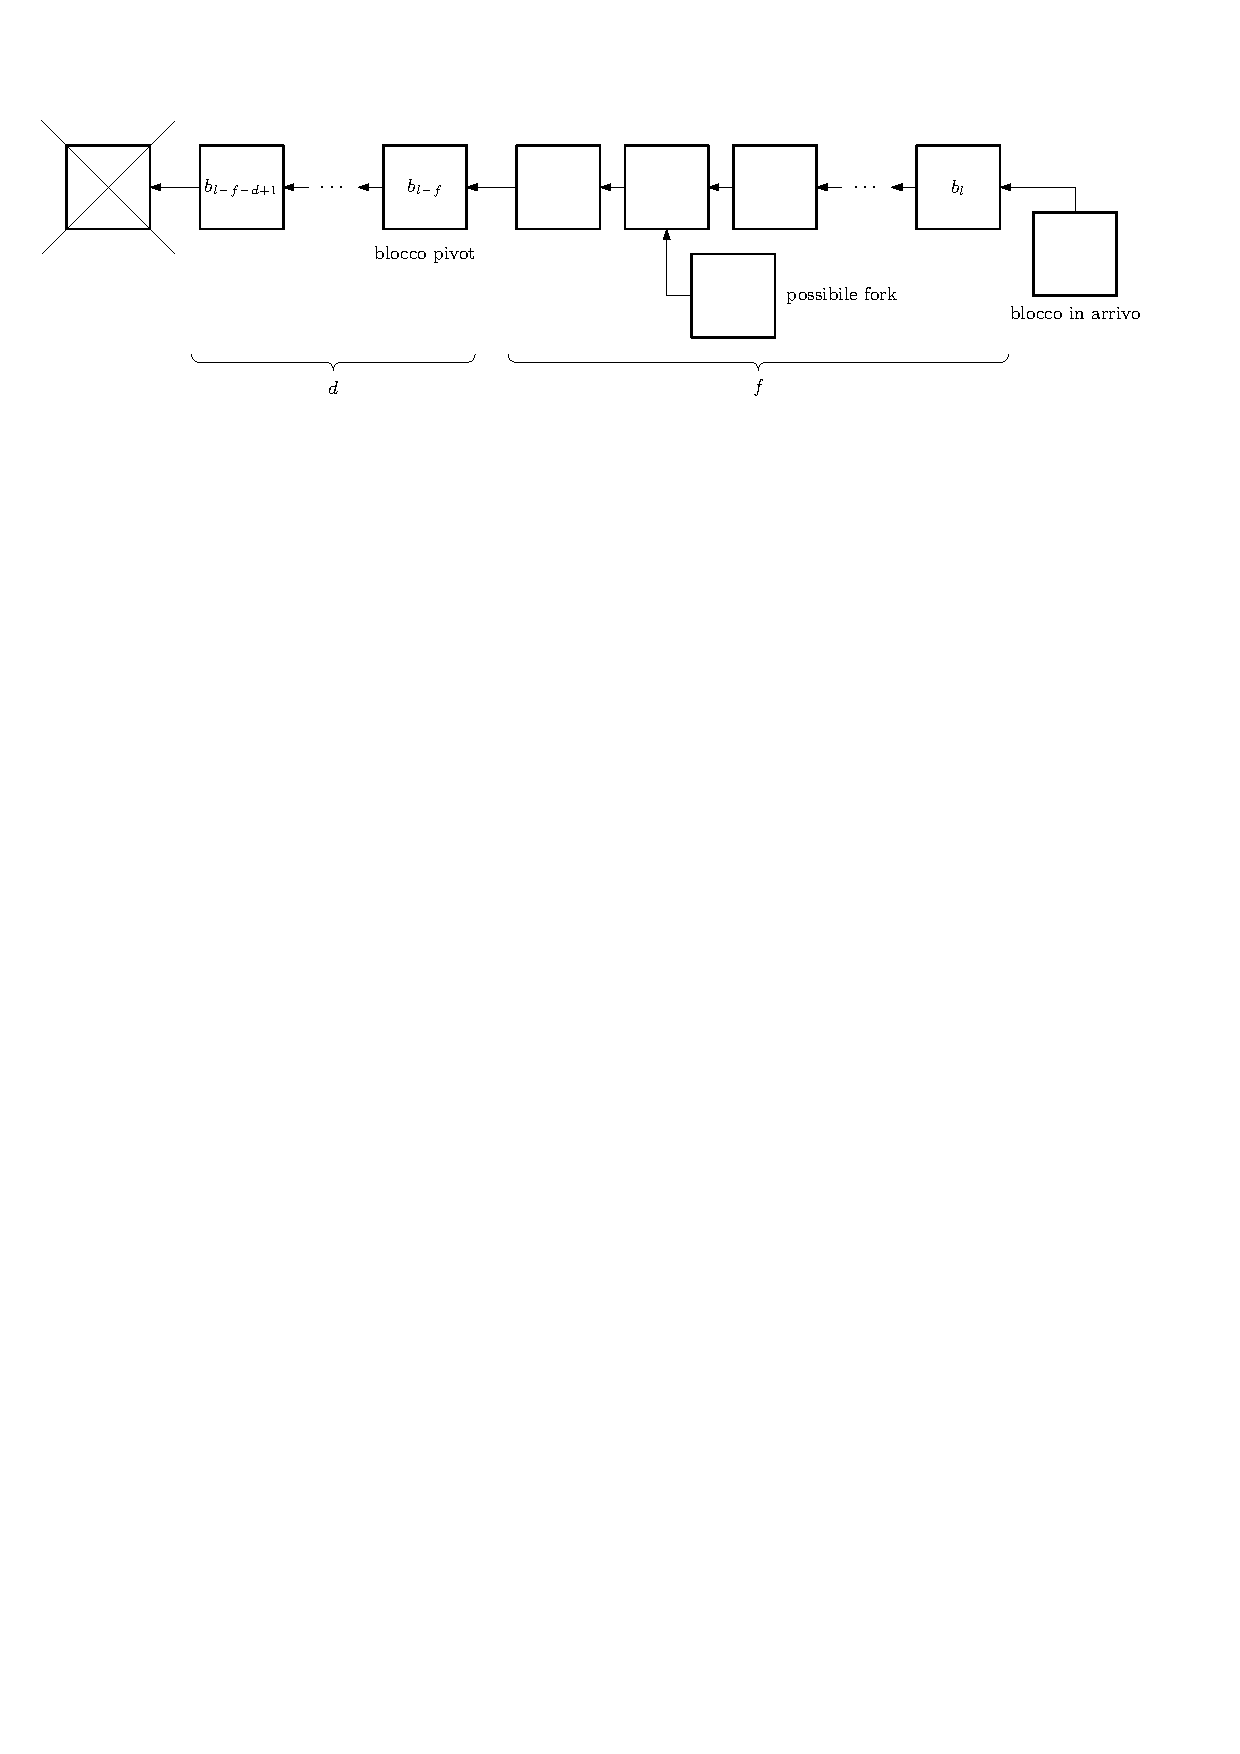
\includegraphics[scale=0.7]{img/capdue/truncated_blockchain.pdf}
	\caption{Blockchain troncata: un nodo memorizza solo gli ultimi $d+f$ blocchi. \emph{Fonte~\cite{bernardini2019blockchains}}}
	\label{fig:blockchain_bern}
\end{figure}

In questo caso si sceglie come blocco pivot $b_{l-f}$, dove $l$ è l'indice dell'ultimo blocco in $\Lambda_N$. Ogni blocco $b_i \in \Lambda_N$ oltre a contenere le transazioni confermate, in una struttura dati autenticata come le altre blockchain (ad esempio Bitcoin), include anche il pADS $\tau_i$, che rappresenta lo stato prima dell'applicazione delle transazioni in $b_i$, che coinvolge solo gli elementi di stato $E_i$ modificati dalle transazioni in $b_i$, il resto è potato, come rappresentato in Figura~\ref{fig:block_content}. Si denota inoltre $\pi_i$ il pADS ottenuto da $\tau_i$ applicando le transazioni in $b_i$: $\pi_i$ non necessita di essere memorizzato e può essere calcolato \emph{al volo} quando è necessario.

\begin{figure}
	\centering
	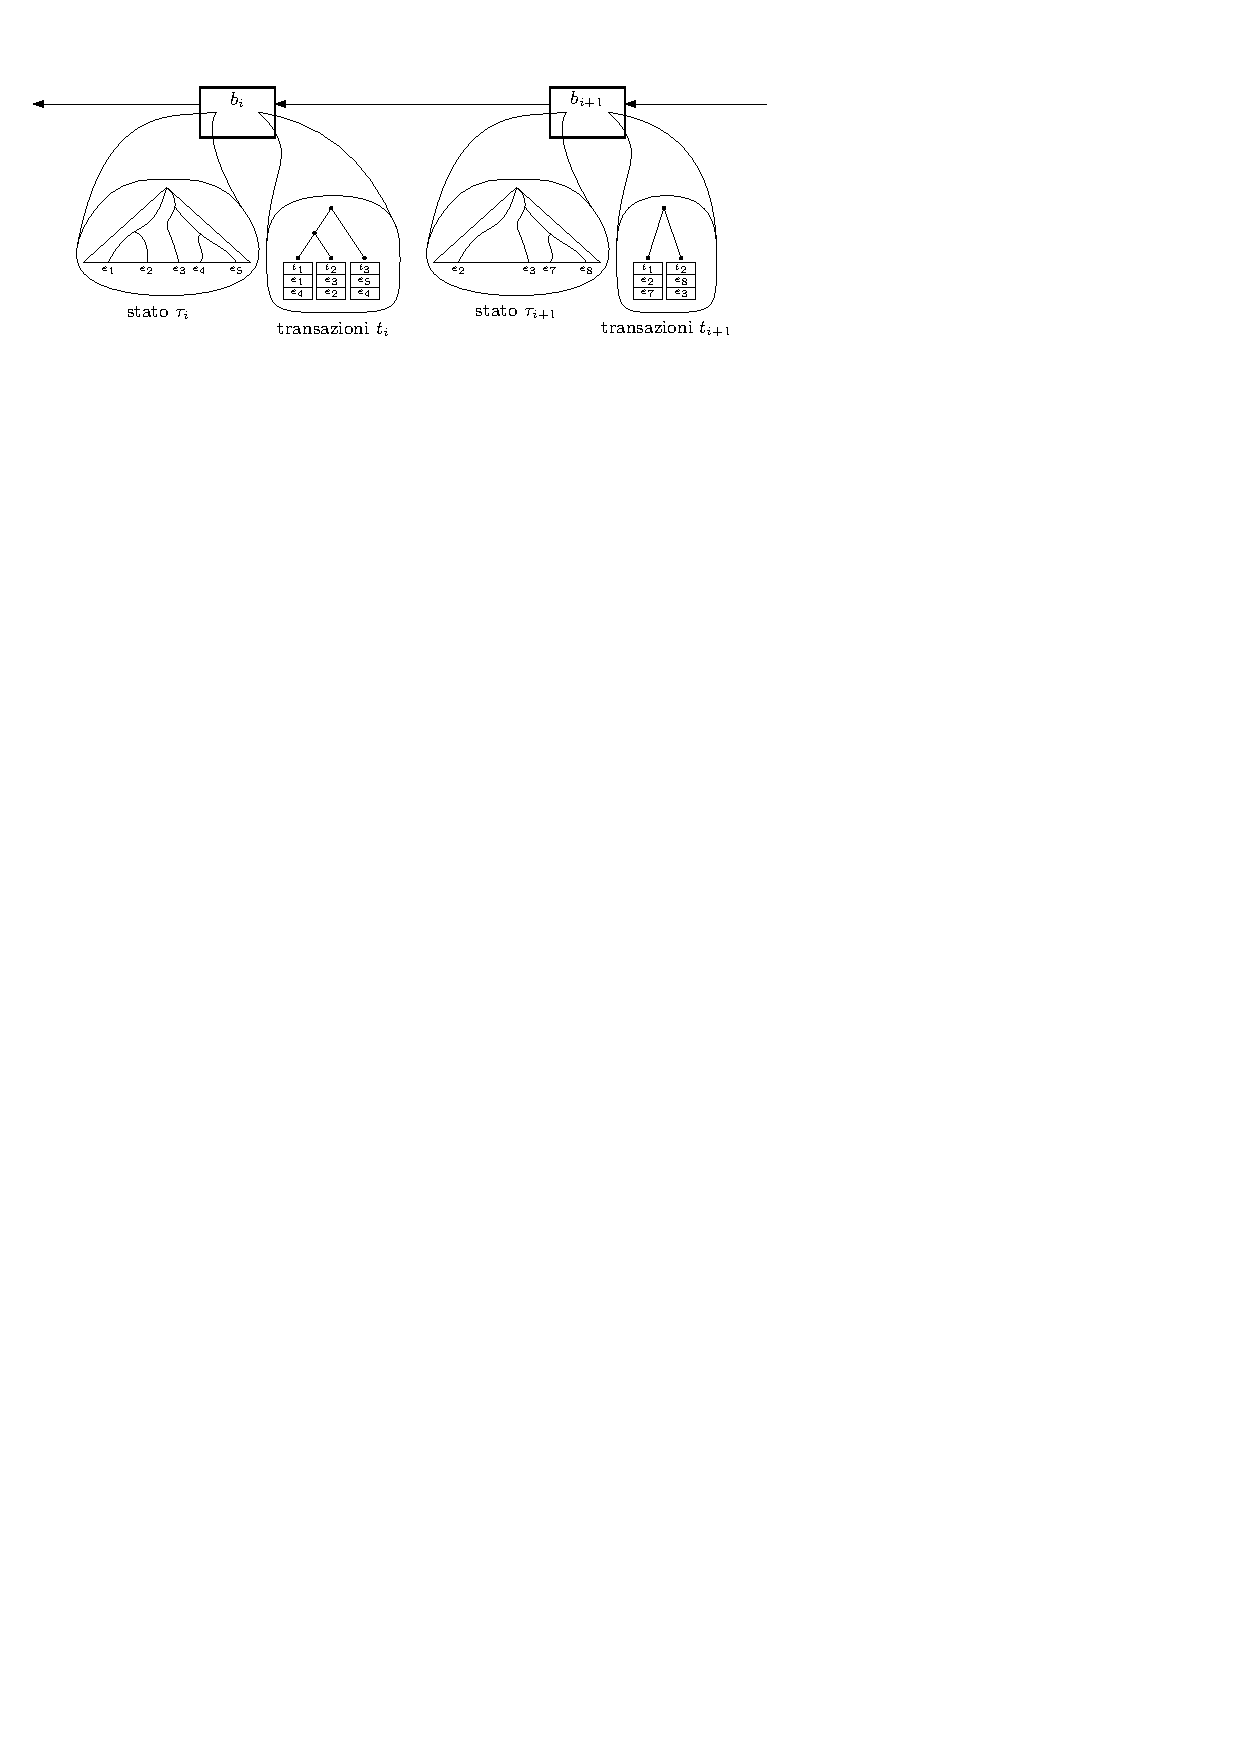
\includegraphics{img/capdue/block_bern.pdf}
	\caption{Contenuto di un blocco. Ognuno blocco $b_i$ contiene le transazioni confermate $t_i$ e il Merkle Tree potato $\tau_i$ contenente solo le foglie degli elementi di stato modificati in $t_i$. \emph{Fonte~\cite{bernardini2019blockchains}}}
	\label{fig:block_content}
\end{figure}

Per la creazione del prossimo blocco $b_{l+1}$ da inserire in blockchain, vengono selezionate tutte le transazioni in attesa dal pool di transazioni. Per ogni elemento di stato $e \in E_{l+1}$, si verifica l'integrità di $\delta_i(e) = \langle v, p, i \rangle$, imponendo $i \geq l-f-d+1$ (in caso contrario la transazione sarebbe troppo vecchia), e comparando il root-hash calcolato da $p$ e da $v$, secondo quanto descritto nel Paragrafo~\ref{sec:ads}, con il root-hash di $\tau_i$ contenuto nel blocco $i$. Se una delle due condizioni non è valida, le transazioni che coinvolgono quell'elemento di stato vengono scartate.
Per il calcolo di $\tau = \tau_{l+1}$, rappresentante lo stato prima dell'applicazione delle transazioni nel futuro blocco $b_{l+1}$ si procede secondo l'Algoritmo~\ref{alg:tau_compute}.
Sia $\delta$ la lista contenente tutte le $\delta_i(e)$ per ogni $e \in E_{l+1}$. Inizialmente si effettua un merge delle proof contenute in $P$, ottenuta estraendole da $\delta$, considerando solo la topologia e non gli hash. Poi si itera partendo da $x = l$ decrementandola fino all'indice del blocco più vecchio, eseguendo per ogni iterazione le seguenti operazioni: (1) si riempiono i nodi di $\tau$ ancora vuoti con $\pi_x$, e (2) la stessa cosa con $\delta_x$, mediante la procedura \emph{fillEmpty}. La procedura si ripete finche $\tau$ non è pieno. La correttezza di \emph{computeState} è data dal fatto che si da precedenza ai nodi più aggiornati nel tempo, mentre gli hash non presenti in $\pi_x$, poiché gli elementi di stato relativi non sono stati modificati nelle transazioni contenute nel blocco $b_x$, sono ottenuti da $\delta_x$.
A questo punto, dopo aver ottenuto lo stato attuale $\tau_{l+1}$ si verifica che ogni transazione $t$ da includere nel blocco rispetta le regole di consenso (ad esempio, non effettua double spending) e la inserisce in $b_{l+1}$. Si esegue l'algoritmo di consenso distribuito e si invia in broadcast il nuovo blocco.
\begin{algorithm}
	\caption{Calcolo di $\tau$}
	\begin{algorithmic}
		\Procedure{computeState}{$\delta$}
			\State{$P \leftarrow$\Call{map}{snd, $\delta$}}
			\State{$\tau \leftarrow$\Call{topologicalMerge}{$P$}}
			\For{$ x \leftarrow l$ \textbf{down to} $l-f-d+1$}
				\State \Call{fillEmpty}{$\tau, \pi_x$}
				\State \Call{fillEmpty}{$\tau, \delta_x$}
				\If{\Call{isFull}{$\tau$}}
					\State{\textbf{break}}
				\EndIf
			\EndFor
			\Return $\tau$
		\EndProcedure
	\end{algorithmic}
	\label{alg:tau_compute}
\end{algorithm}

Alla ricezione del nuovo blocco $b_{l+1}$ un nodo confronta il root-hash ottenuto da $\pi_l$ con il root-hash di $\tau_{l+1}$.  Ogni transazione $t \in b_{l+1}$ viene validata secondo le regole di consenso, utilizzando $\tau_{l+1}$. Se tutte le regole di consenso sono rispettate, $b_{l+1}$ viene inserito, mentre $b_{l-d-f+1}$ viene rimosso da $\Lambda_N$. Il nuovo pivot diventa $b_{l-f+1}$ ed i nodi di storage applicano le transazioni contenute in $b_{l-f+1}$ a $\tau_{l-f+1}$, aggiornando autonomamente le proprie pADS.

\section{Sharding}\label{sec:sharding}

Un'altra proposta in letteratura per risolvere il blockchain scalability trilemma è lo \emph{sharding}, una tecnica impiegata nei database distribuiti, che consiste nel partizionare lo stato della blockchain in molteplici \emph{shard}, gestite in parallelo da differenti sottoinsiemi di nodi, in modo da ridurre l'overhead dei protocolli di consenso e consentire un processamento delle transazioni parallelo tra i vari shard, aumentando il throughput complessivo del sistema e diminuendo il tempo di conferma di una transazione.
Esempi di blockchain che utilizzano questa tecnica sono Elastico~\cite{luu2016secure}, OmniLedger~\cite{kokoris2018omniledger} e RapidChain~\cite{zamani2018rapidchain}.

I protocolli che fanno uso dello sharding in ambito database hanno l'obiettivo di migliorare le performance in ambiente distribuito~\cite{cattell2011scalable, corbett2013spanner}.
Tuttavia essi non possono essere estesi alle blockchain, poiché gli ambiti di impiego sono opposti: mentre nei database, si assume come modello di fallimento quello secondo cui un nodo può non rispondere a richieste o per un problema hardware (come ad esempio, assenza di corrente elettrica, problemi di rete, danneggiamento di hard disk) o per un problema software (ad esempio per un crash del programma), in ambito blockchain l'ambiente di esecuzione è più ostile. Infatti i nodi, oltre che danneggiarsi, possono adoperare comportamenti malevoli.

Gli aspetti fondamentali di una blockchain sharded che ne garantiscono correttezza e sicurezza sono: (1) selezione periodica e randomica dei nodi che compongono una shard con metodologie resilienti ad attacchi di tipo Sybil, e (2) gestione delle transazioni \emph{cross-shard}, in cui gli input ed output riguardano due o più shard.

\paragraph*{Modello di riferimento}
In OmniLedger, la rete è composta da $n$ \emph{validatori}, con il compito di processare le transazioni generate dagli utenti del sistema. Gli $n$ validatori sono uniformemente distribuiti tra $m$ shard, i quali processano solo una parte delle nuove transazioni. Denotato $s_i$ ed $s_j$ le transazioni processate dagli shard $i$ e $j$ rispettivamente, con $i, j \in \{1,\dots,m\}$, e $i \neq j$, $s_i$ ed $s_j$ sono due insiemi disgiunti. Ogni validatore $i$ ha una coppia chiave pubblica $pk_i$ e privata $sk_i$. Il tempo è suddiviso in intervalli di tempo fissi tra i quali avvengono delle riconfigurazioni degli shard, denominati \emph{epoche}. Ogni epoca è composta da un certo numero di \emph{round} nei quali ogni shard processa le transazioni di cui è responsabile. Per partecipare all'epoca $e$, un validatore deve registrarsi entro la fine dell'epoca $e-1$, secondo un procedimento che stabilisca la sua identità resiliente ad attacchi Sybil. Esiste infatti una blockchain che contiene le identità di tutti i validatori registrati. Infine si denota con $f$ il numero di validatori Bizantini, tale che $n = 4f$, ovvero al massimo il $25\%$ dei validatori è malevolo. Il modello di RapidChain è simile, con $f \leq 33\%$.

\paragraph*{Formazione di uno shard}
La formazione degli shard di cui è composta la rete, affinché sia sicura, viene effettuata randomicamente, sulla base di un numero random senza alcun bias e imprevedibile. Mentre alcuni sistemi~\todo{citare sistemi sharded con beacon per generazione numeri random} utilizzano un \emph{beacon} fidato per la generazione di numeri random, altri, come OmniLedger e RapidChain, si basano su un generatore di numeri casuali distribuito. Il primo si basa sulla combinazione del protocollo RandHound~\cite{syta2017scalable} e VRF~\cite{micali1999verifiable}, mentre il secondo si basa su Verifiable Secret Sharing (VSS)~\cite{pedersen1991non}.
RandHound si affida ad un leader per l'orchestrazione del protocollo: se la sua elezione fosse deterministica, un utente malevolo può sfruttare la situazione a proprio vantaggio e portare fino a $fn$ fallimenti. La selezione è quindi randomica, mediante l'uso della VRF. Ogni validatore $i$ genera un valore $t_{i,e,v} =$VRF$_{sk_i}("leader" || config_e || v)$, dove $config_e$  è la lista contenente tutti i validatori registrati per l'epoca $e$ e $v$ è un contatore. Ogni validatore invia il proprio $t_{i,e,v}$, selezionando il minore che riceve e accettando il corrispondente come leader. Se il leader fallisce nell'iniziare la procedura di RandHound, $v$ viene incrementato e riparte la selezione. Il leader genera mediante RandHound ed invia in broadcast a tutti i validatori un numero random $rnd_e$ insieme alla sua prova di correttezza. $rnd_e$ verrà utilizzato da ogni validatore per determinare lo shard a cui è stato assegnato.
Dal punto di vista della sicurezza, un utente malevolo può essere selezionato come leader. Egli può scegliere di cooperare al protocollo, oppure di fallire, venendo escluso per tutta l'epoca $e$. Si noti che non può generare più numeri casuali e proporre quello che più lo soddisfa (ad esempio, un numero tale che porti ad una permutazione in cui tutti i nodi malevoli sono in uno shard), poiché questo dipende da $v$. Infine, la probabilità che un utente onesto sia selezionato dopo che un utente malevolo abbia vinto la lotteria, è molto alta, poiché la probabilità che l'utente malevolo sia selezionato $a$ volte di fila, decresce esponenzialmente con $a$, secondo $(f/n)^a$.
Per diminuire l'impatto di attacchi del tipo \emph{join-leave}, in cui un utente malevolo che entra a far parte di uno shard si disconnette durante l'epoca $e$, viene effettuato uno swap periodico dei nodi tra uno shard e l'altro, spostando solamente $k = \log \frac{n}{m}$ nodi alla volta, per diminuire l'overhead necessario alla risincronizzazione dei nodi che cambiano shard. La risincronizzazione consiste nel download della blockchain dello shard. Per ridurre la dimensione si può attuare un meccanismo di potatura/checkpoint come in~\cite{bernardini2019blockchains, kokoris2018omniledger, leung2019vault}. In RapidChain, un nodo scarica solo l'insieme delle \emph{unspent transaction} (UTXO) di uno shard, sufficienti a verificare le future transazioni.

\paragraph*{Comunicazione cross-shard}
Lo sharding permette di ridurre lo spazio richiesto dalla blockchain, ma allo stesso tempo aumenta la difficoltà della verifica delle transazioni, perché gli input e gli output possono risiedere su shard differenti. Sia $t$ la transazione generata da un utente. $t$ ha un numero $N$ di input $I_1, \dots, I_N$ e un output $O$. Senza perdità di generalità, si può considerare che ad ogni input corrisponda un unico shard.\todo{da rivedere la frase, forse non si capisce bene} Quindi, si denotano gli shard di input ed output con $C_{in}^j$, tale che $j \in \{1, \dots, N\}$, e con $C_{out}$, rispettivamente. 
In OmniLedger, per processare ogni transazione $t$ in modo atomico tra shard, si utilizza un protocollo denominato \emph{Byzantine Shard Atomic Commit}, al cui termine $t$ è o confermata o abortita. Il protocollo è formato da 3 step (vedi Figura~\ref{fig:atomix}):

\begin{figure}
	\centering
	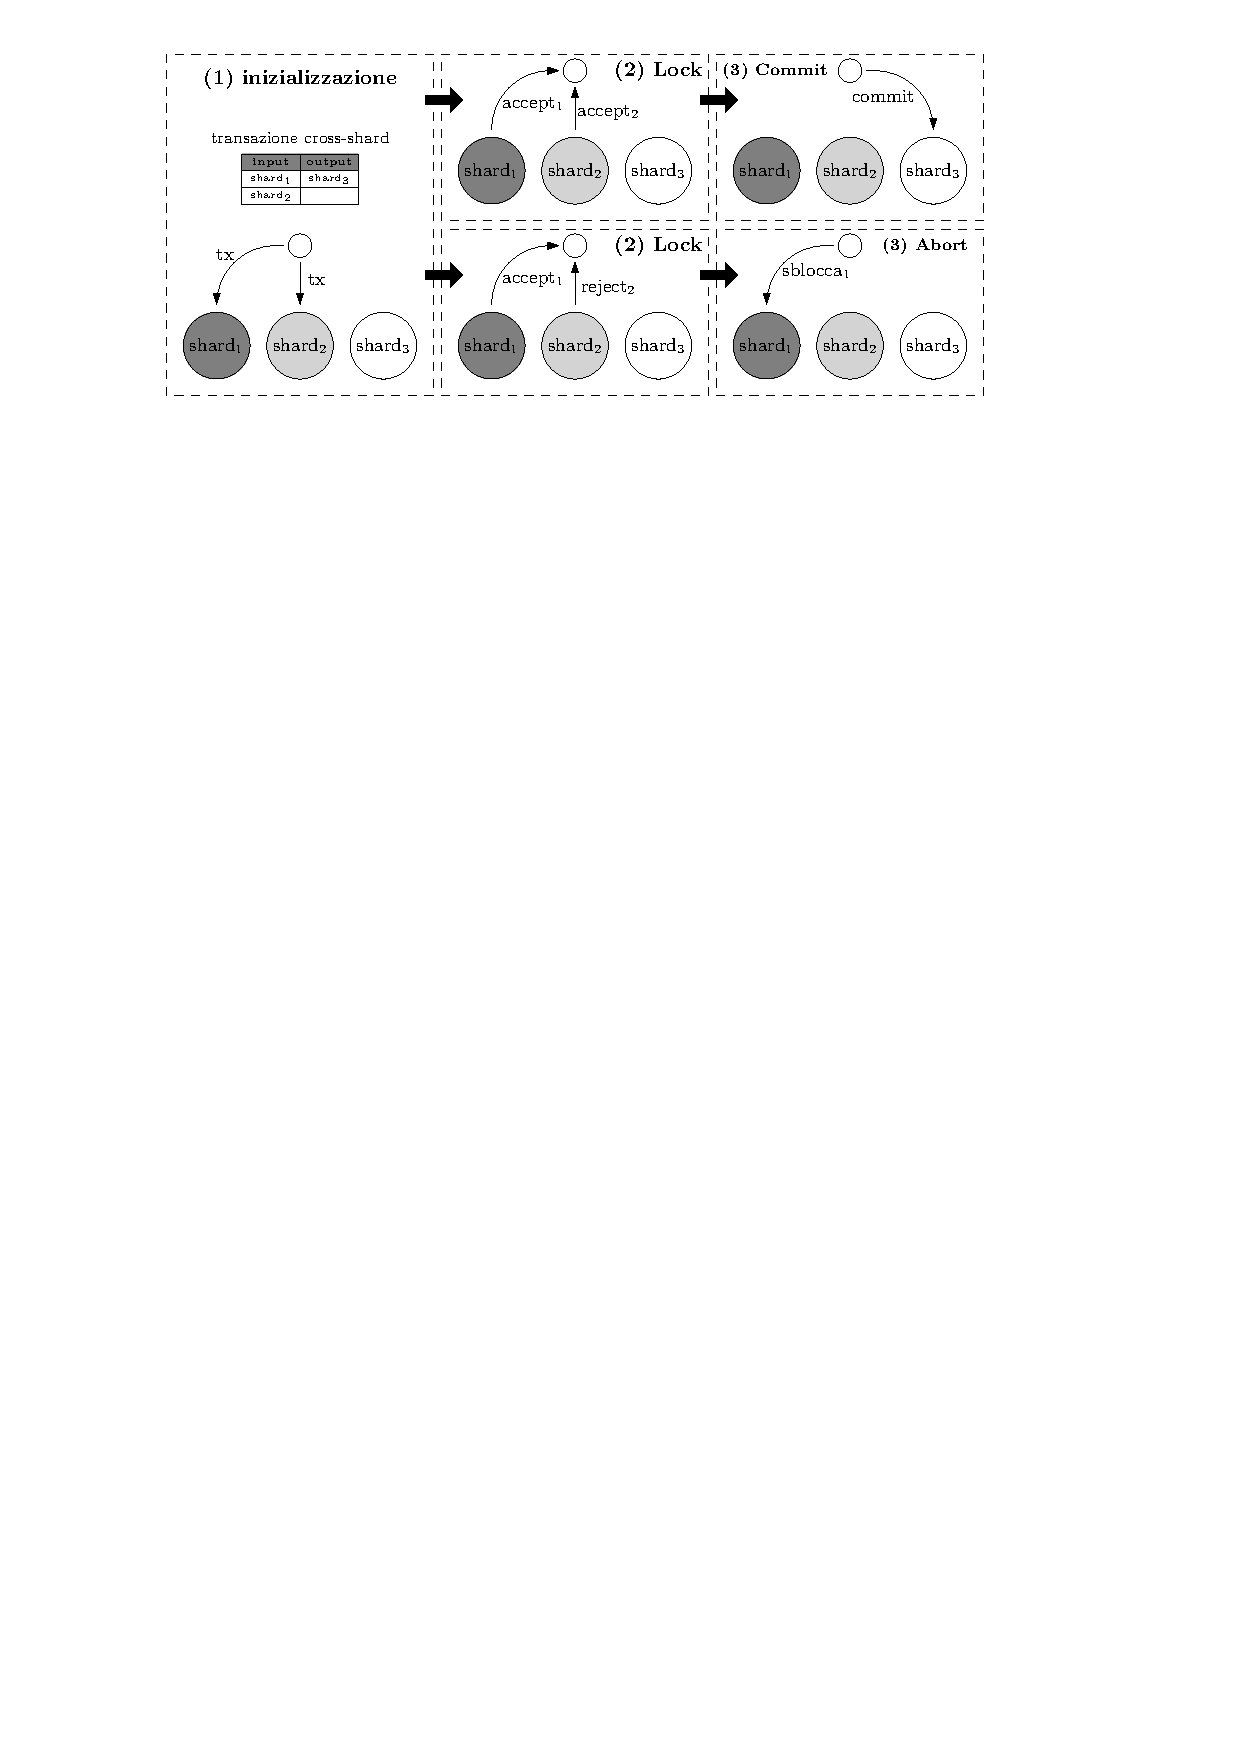
\includegraphics[scale=0.9]{img/capdue/atomix.pdf}
	\caption{Processamento di una transazione cross-shard in Omniledger. \emph{Fonte~\cite{kokoris2018omniledger}}}
	\label{fig:atomix}
\end{figure}

\begin{enumerate}
	\item \textbf{Inizializzazione}: il client $c$ invia $t$ a tutte i $C_{in}^j$ per ogni input $j$ $I_j$ in $t$.
	\item \textbf{Lock}: Ogni leader di $C_{in}^i$ verifica la validità della transazione, ovvero se l'input di cui è responsabile $C_{in}^i$ è spendibile. Se la transazione è valida, il leader imposta la UTXO associata come spesa (quindi bloccata), ed invia a $c$ una \emph{proof-of-acceptance}, ovvero una proof di un Merkle Tree del blocco in cui la transazione è stata inserita. Se non è valida, $c$ riceve una \emph{proof-of-rejection}.
	\item \textbf{Unlock}: in base alla precedente fase il client può confermare o abortire la transazione:
	
	\begin{enumerate}
		\item \textbf{Unlock to commit}: se tutti i $C_{in}^i$ rispondono con una \emph{proof-of-acceptance}, $c$ può confermare la transazione. Crea quindi una transazione \emph{unlock-to-commit} destinata a $C_{out}$ contenente tutte le \emph{proof-of-accemptance} per ogni input e $C_{out}$ crea una nuova UTXO destinata all'output di $t$;
		\item \textbf{Unlock to abort}: se riceve almeno una \emph{proof-of-rejection}, $c$ può richiedere di sbloccare le UTXO per gli input $I_j'$ per i quali ha ricevuto una \emph{proof-of-acceptance}. $c$ crea quindi una transazione \emph{unlock-to-abort} dove inserisce almeno una \emph{proof-of-rejection} per un input in modo tale da sbloccare la UTXO associata.
	\end{enumerate}

\end{enumerate}

Questa soluzione non richiede una comunicazione inter-sharding, ma genera un grande overhead di comunicazione dovuta ad ogni proof generata per ogni input della transazione $t$. Inoltre, un altro aspetto negativo è che richiede del lavoro aggiuntivo, rispetto alla semplice e sola creazione di una transazione, al client, rendendolo più difficile da utilizzare per dispositivi semplici, come quelli IoT.

RapidChain risolve questo problema nel modo seguente. L'utente che crea $t$, invia $t$ a $C_{out}$\footnote{secondo un meccanismo di \emph{inter-committee routing} molto efficiente basato sull'algoritmo di routing di Kademlia~\cite{maymounkov2002kademlia}}. Il leader di $C_{out}$ per ogni input $I_j$ di $t$, genera una transazione $t_i$ con input $I_j$ ed output $I_j'$, con $|I_j| = |I_j'|$ (con lo stesso valore) e $I_j'$ è diretta sul conto di $C_{out}$. Infine genera la transazione $t_{N+1}$, avente input $I_j'$, con $j \in \{1, \dots, N\}$ e output $O$. Il leader invia $t_i$ ad ogni $C_{in}^i$ e se $t_i$ è confermata, $C_{in}^i$ invia $I_i'$ a $C_{out}$. Se tutte le transazioni $t_i$, con $i \in \{1, \dots, N\}$ sono confermate, allora $C_{out}$ inserisce $t_{N+1}$ nella propria blockchain.


\paragraph*{}
Sebbene lo sharding possa rappresentare una soluzione alla scalabilità, in modo da migliorare l'utilizzo dell'hash power complessivo della rete e ridurre l'overhead di storage per la memorizzazione dell'intero stato della blockchain, la sicurezza può essere un problema: è più facile per un attaccante prendere il controllo di una singola shard, a causa del ridotto numero di partecipanti presenti nello shard stesso, secondo l'attacco noto in letteratura come \emph{1\% attack}, o \emph{single-shard  takeover attack}~\cite{chauhan2018blockchain}. Secondo questo attacco, per una rete composta da $m=100$ shard, ad un attaccante è necessario solo l'1\% dell'hash power totale per attuare i suoi comportamenti malevoli, come quelli descritti nel Paragrafo~\ref{attacks}.
\chapter{Una soluzione scalabile}

In questo capitolo viene presentata da un punto di vista teorico, l'architettura progettata ed analizzata in questo lavoro di tesi, in grado di risolvere il blockchain scalability trilemma. In particolare, inizialmente si analizzeranno le problematiche negli approcci correnti, per poi descrivere l'architettura, mostrando il ruolo di ciascun nodo e descrivendo il flusso di informazioni scambiato tra i nodi della rete. Infine si dimostrerà la correttezza dell'architettura e la sua scalabilità, con gli omonimi teoremi.
L'architettura è stata proposta in letteratura nell'articolo \emph{Scaling Blockchains Without Giving up Decentralization and Security (A solution to the Blockchain Scalability Trilemma)}~\cite{del2020scaling}.

\section{Problematiche in approcci correnti}

I sistemi correnti presentano aspetti che rendono le blockchain non scalabili. In particolare le tre criticità individuate sono:

\begin{enumerate}
	\item le nuove transazioni vengono inviate in broadcast a tutti i nodi della rete;
	\item ogni nuovo blocco è ricevuto da tutti i nodi;
	\item esiste un insieme dei nodi che processano tutte le nuove transazioni da includere nel prossimo blocco.
\end{enumerate}

Questi aspetti implicano che per poter processare un quantitativo di transazioni maggiori, si deve aumentare proporzionalmente la capacità computazionale e la banda dei singoli nodi (scalabilità \emph{verticale}). \'E preferibile invece una scalabilità \emph{orizzontale}, secondo cui per far fronte all'aumento di transazioni da processare si aggiungono nuovi nodi alla rete.

Nella presente tesi, l'obiettivo è quello di progettare un'architettura che affronti i tre problemi prima menzionati, tralasciando gli aspetti legati alla scalabilità del protocollo di consenso distribuito. Infatti i tre aspetti sono del tutto indipendenti da quest'ultimo e sono rilevanti anche per protocolli di consenso \emph{light}~\cite{poon2016bitcoin}. Si tralasciano gli aspetti legati allo storage dello stato della blockchain, poiché affrontato in altri lavori, come presentato nel Paragrafo~\ref{sec:bernardini}.

In letteratura, alcune proposte di architettura scalabile introducono lo \emph{sharding}, descritto nel Paragrafo~\ref{sec:sharding}. Tuttavia, come si è visto, assicurare l'atomicità delle transazioni è impegnativo in contesti in cui queste riguardano più shard (transazioni \emph{cross-shard}), che richiedono tecniche simili al 2PC o creazione di ulteriori transazioni per ogni input presente in quella originaria. Altra criticità, più importante, riguarda la sicurezza: gli shard piccoli permettono all'architettura di scalare, ma sono meno sicure rispetto ad una blockchain formata da tutti i nodi della rete.


\section{Aspetti centrali e definizioni di base}

Per semplicità si assume che la blockchain realizzi un sistema di cripto-valute, in cui ad ogni \emph{indirizzo} (o \emph{conto}) è associato un saldo non negativo e le transazioni spostano del valore monetario da un conto all'altro, modificando di conseguenza il saldo su entrambi gli indirizzi.

Si definiscono \emph{transazioni candidate}, le transazioni generate dagli utenti ma ancora non processate dalla blockchain. Una transazione è \emph{confermata}, o \emph{accettata} se è stata processata dalla blockchain ed è inclusa in un blocco.

L'insieme delle transazioni candidate rappresenta il carico della blockchain, identificato dalla frequenza misurata in transazioni al secondo. Si assume che, il carico delle transazioni candidate sia distribuito uniformemente sullo spazio degli indirizzi. Il tempo impiegato a confermare una transazione candidata è denominato \emph{latenza}. Si definisce \emph{throughput massimo} della blockchain la massima frequenza delle transazioni candidate che è possibile confermare con latenza limitata. Quando il carico è minore del \emph{massimo throughput} si dice che il sistema è \emph{well-provisioned}.
Si dice che un'architettura blockchain \emph{scala} se, partendo da una blockchain well-provisioned, la blockchain rimane well-provisioned incrementando proporzionalmente carico e nodi nella rete.


Per i problemi presentati precedentemente, il \textit{blocco} dell'architettura proposta non è come quello delle soluzioni comuni, in cui sono memorizzate le transazioni confermate dai miner. Infatti in quest'ultimo caso la dimensione del blocco dipende dal numero di transazioni confermate e quindi dal carico generato dalla rete. Questo ovviamente è un problema di scalabilità, per cui la dimensione del blocco è costante e contiene solamente l'hash del blocco precedente e l'hash dello stato della blockchain dopo l'applicazione delle transazioni del blocco. Per cui, il blocco può esser visto come l'header del blocco delle soluzioni tradizionali. L'hash dello stato è ottenuto dal root-hash del Merkle Tree dello stato, per cui è chiamato \emph{state root-hash}.

L'intera architettura, per ragioni di scalabilità, è organizzata secondo una \emph{pipeline}, in cui ogni operazione è eseguita in diversi \emph{stage}. Il tempo è inoltre suddiviso in \emph{round}, numerati sequenzialmente. In ogni round ogni nodo può partecipare alla conferma delle nuove transazioni oppure alla creazione del nuovo blocco. L'ultimo stage della pipeline corrisponde alla creazione del nuovo blocco, inviato in broadcast a tutti i nodi della rete.

Le operazioni vengono eseguite da un certo numero di \emph{comitati}, che lavorano insieme per la validazione e conferma delle nuove trasazioni e per la creazione del corrispettivo blocco per ogni round. Ogni comitato è formato da un numero di \emph{membri}, che è costante, come si vedrà in seguito, anche all'aumentare dei nodi sulla rete. \'E importante, per problemi di sicurezza, che i membri di ogni comitato, come nell'approccio sharded (vedi Paragrafo~\ref{sec:sharding}), siano selezionati in modo randomico e cambiati regolarmente, per esempio ad ogni round. Un approccio può essere quello proposto da Algorand~\cite{gilad2017algorand}, in cui si utilizzano le VRF~\cite{micali1999verifiable}. I comitati cooperano quindi alla conferma e creazione del nuovo blocco, comunicando mediante un meccanismo di comunicazione \emph{inter-committee}, discusso in seguito.
Ogni comitato svolge il proprio ruolo durante uno stadio e invia il risultato del lavoro ai membri dei comitati dei successivi round/stadi.

Si denota con $B_i$ il blocco prodotto come output dell'ultimo stadio nel round $i$, mentre con $B^i$ il blocco che contiene le transazioni che entrano nella pipeline nel round $i$. Se la pipeline ha $q$ stadi, le transazioni che entrano nella pipeline al round $i$, e che sono accettate, faranno parte del blocco prodotto dal comitato dell'ultimo stadio al round $i+q-1$. Quindi, $B^i = B_{i+q-1}$. Le transazioni confermate in $B^i$ saranno visibili a tutti i nodi della rete a partire dall'inizio del round $i+q$.

Differentemente da altre sistemi presentati nei precedenti paragrafi, l'intero stato della blockchain non viene memorizzato da ogni nodo, non solo per le eccessive dimensioni richieste che aumentano nel tempo, ma anche perché richiede un processamento da parte di ogni nodo proporzionale al carico. Come è stato descritto nel Paragrafo~\ref{sec:bernardini}, un nodo può creare e partecipare alla conferma di un insieme di transazioni anche senza dover memorizzare l'intero stato. Infatti, esso è memorizzato in una DHT, dove ogni nodo, denominato \emph{storage node}, ne memorizza solo una parte, quello per cui è \emph{autorità}. Sulla DHT è costruito un Merkle Tree $W$ \emph{virtuale} sull'intero spazio degli indirizzi, in cui ogni foglia è un indirizzo. Gli storage node memorizzando solo una parte dello stato, ovvero un sottoinsieme degli indirizzi, posseggono solo una parte di $W$ (pADS), che è potato e ha per foglie gli indirizzi per cui esso è \emph{autorità}.

Come descritto nel Paragrafo~\ref{sec:bernardini}, un nodo $n$ che crea una transazione ha la responsabilità di fornire le prove crittografiche dei conti associati agli indirizzi che sono coinvolti nella transazione e che la stessa modifica. Il nodo $n$ ottiene le prove crittografiche dagli storage node autorità per gli indirizzi coinvolti nella nuova transazione. Poiché ogni storage node possiede una versione potata del Merkle Tree $W$, può fornire tali prove per gli indirizzi che memorizza. Tuttavia i conti e le rispettive prove sono indietro nel tempo rispetto a quando verranno confermate dagli opportuni comitati. Si dice quindi che una proof $p$ è \emph{relativa} ad uno stato della blockchain ottenuto applicando le transazioni nel blocco $B$, intendendo che è valida rispetto allo state root-hash contenuto nel blocco $B$. In modo più semplice, si può dire che $p$ è relativa a $B$.
Ogni nodo della rete, memorizza solo gli ultimi $d$ blocchi che ha ricevuto, per cui possiede i blocchi $B_{i-1}=B^{i-q}, \dots, B_{i-d}=B^{i-q-d+1}$. Quindi, una proof $p$ relativa a $B_j$ è considerata \emph{scaduta} al round $i$, se $i > j + d$.

Poiché nel round $i$ l'ultimo blocco disponibile è $B_{i-1}$, uno storage node per ogni indirizzo richiesto, risponde con uno stato ed una proof relativa a $B_{i-1}$. Inoltre, visto che nel modello, senza perdere di generalità, un nodo impiega un round per ottenere tutte le proof relative agli elementi di stato coinvolti in una nuova transazione, affinché i comitati del primo stadio della pipeline possano validare le proof relative ai conti coinvolti nelle transazioni, $d \geq 2$.

Infine si assume che non ci siano problemi di rete, per cui ogni nodo riceve tutti i messaggi inviati da un nodo sorgente.

\section{Architettura e ruolo dei comitati}\label{sec:architettura}

In questo paragrafo è descritta l'architettura e il ruolo di ogni comitato dal momento in cui un nodo crea una transazione, fino alla sua conferma. La Figura~\ref{fig:architecture} mostra l'architettura e il flusso di informazioni scambiate tra i comitati.

\begin{figure}
	\centering
	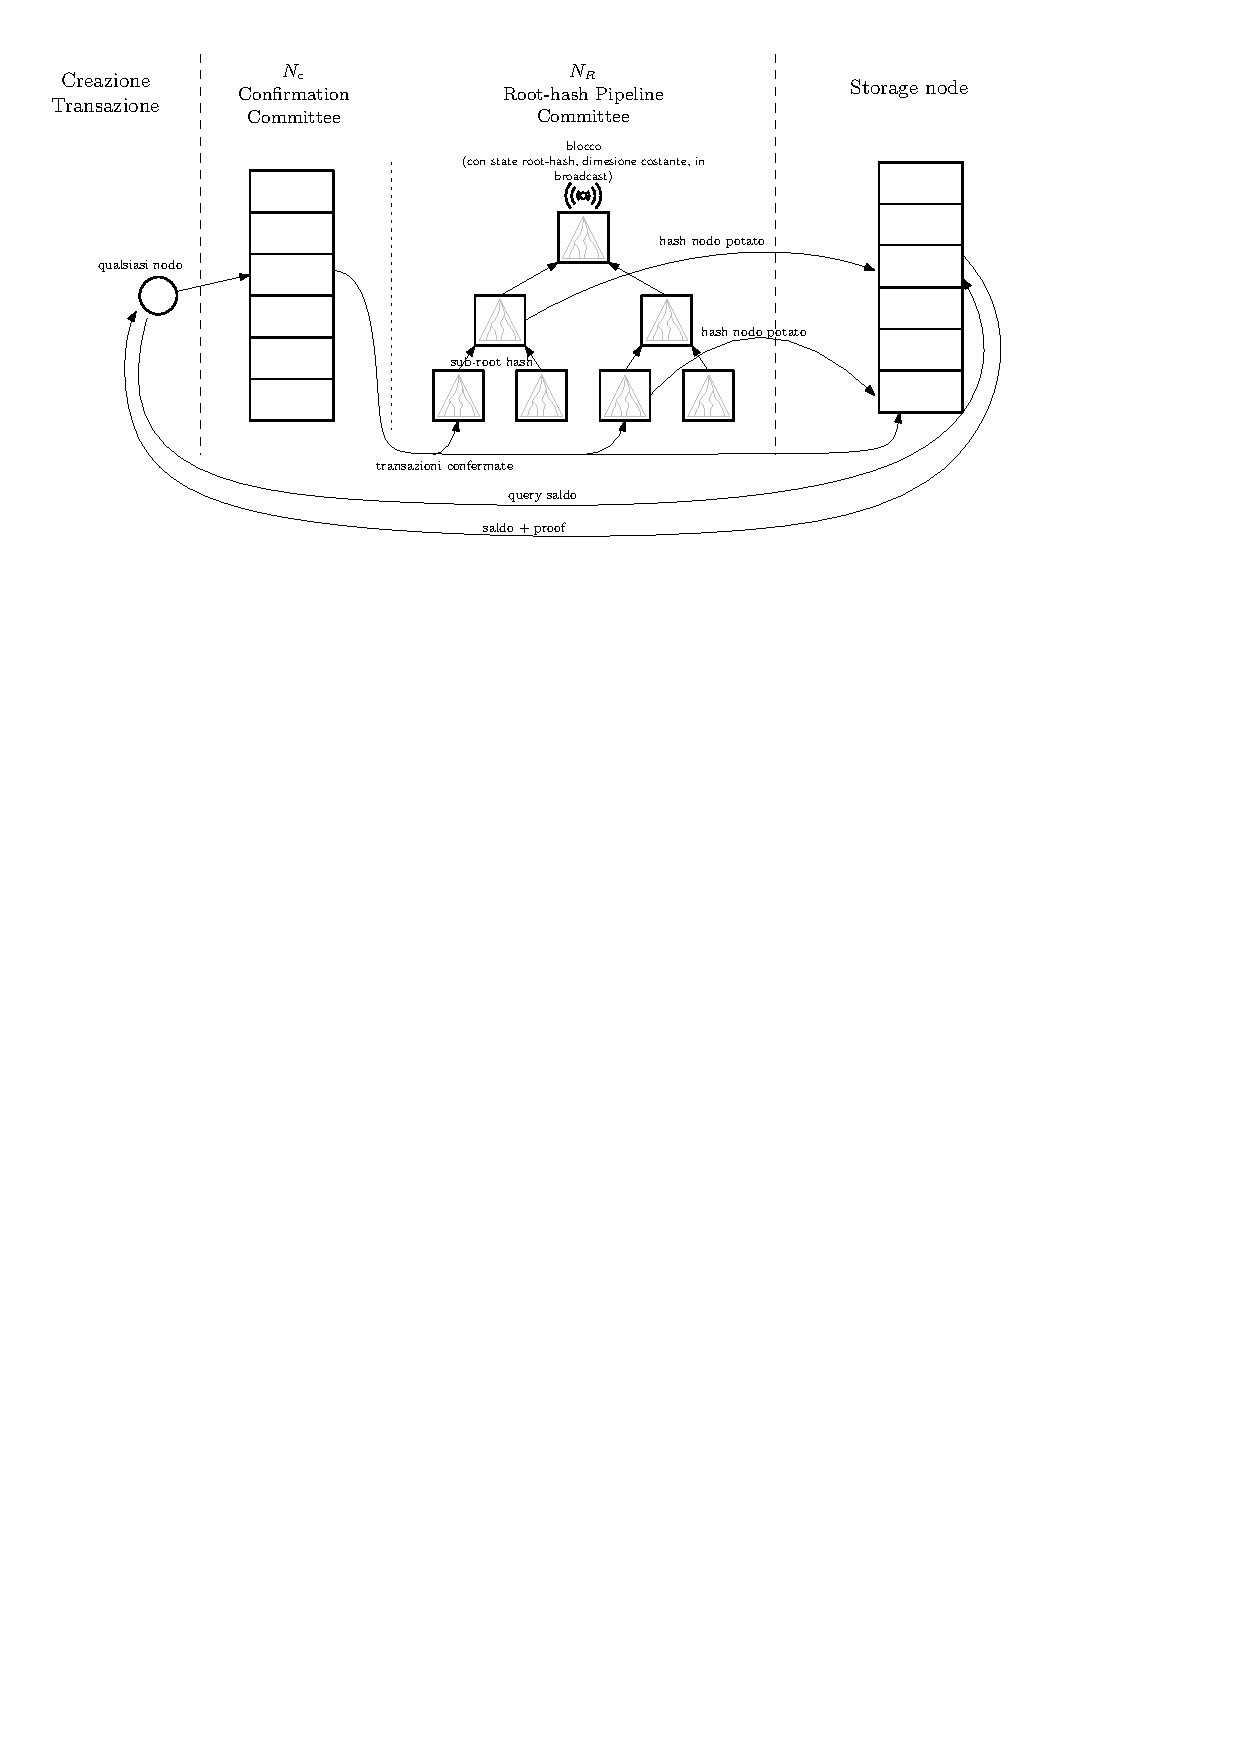
\includegraphics[scale=0.82]{img/captre/bc.pdf}
	\caption{Flusso delle informazioni dell'architettura proposta.}
	\label{fig:architecture}
\end{figure}

Ogni nodo può creare una transazione. Come descritto nel paragrafo precedente, una nuova transazione deve contenere il saldo dei conti associati e le proof di integrità relative, ottenute durante il round precedente dagli storage node autorità per gli elementi di stato coinvolti nella transazione. Le nuove transazioni (candidate) non sono inviate in broadcast come nelle soluzioni tradizionali, ma ad un ristretto numero di nodi.

Il ruolo di validazione e conferma delle nuove transazioni è eseguito dai \emph{Confirmation Committee} (\emph{CC}). Ogni CC è denotato con $C_k$, con $k = 1, \dots, N_c$, dove $N_c$ è il numero di CC. Quando è importante, si denota con $C_k^i$ il $k$-esimo Confirmation Committee relativo al round $i$. Come detto prima, per motivi di sicurezza, ogni Confirmation Committee tra un round e l'altro è formato da membri differenti. Il nodo che crea la transazione $t$, la invia a $C_k^i$ tale che $k = hash(t_s) \mod N_c$, dove $t_s$ è la sorgente della transazione $t$, e si dice che $C_k^i$ è \emph{responsabile} per $t$. Ogni nuova transazione $t$ è ricevuta da $C_k^i$ \emph{prima} dell'inizio del round $i$, in modo tale che $C_k^i$ possa processare $t$ durante il round $i$. L'insieme di transazioni per cui $C_k^i$ è responsabile è denotato $P(C_k^i)$. Si denota con $P^i = \bigcup_k P(C_k^i)$ l'insieme di tutte le transazioni processate da tutti i Confirmation Committee nel round $i$. Il risultato di un $C_k^i$ è una lista di transazioni valide e confermate denotato $A_k^i$, con $A_k^i \subseteq P(C_k^i)$.

$C_k^i$, affinché possa validare correttamente le transazioni, per ogni transazione $t$ ottiene il saldo associato a $B^{i-1}$, in modo da verificare che $t_s$ non diventi negativo applicando la transazione $t$. Poiché le proof fornite in $t$ sono relative a $B_{i-2} = B^{i-q-1}$, esse sono troppo vecchie. Infatti, i conti associati potrebbero essere stati modificati negli ultimi $q$ round, i cui blocchi non sono ancora disponibili (perché la loro creazione è ancora in corso dalla pipeline). Quindi, ogni $C_k^i$ deve conoscere le transazioni confermate, e quindi i cambiamenti allo stato, dai Confirmation Committee dei round precedenti $C_k^{i-q}, \dots, C_k^{i-1}$, ovvero $A_k^{i-q}, \dots, A_k^{i-1}$. Queste transazioni devono essere utilizzate per aggiornare tutti i conti associati alle transazioni in $P(C_k^i)$ per ottenere lo stato di $B^{i-1}$. Questo processo è chiamato \emph{time-updating}. La Figura~\ref{fig:pipeline} mostra la pipeline e riporta gli input forniti ad un generico $C_k^i$.

\begin{figure}
	\centering
	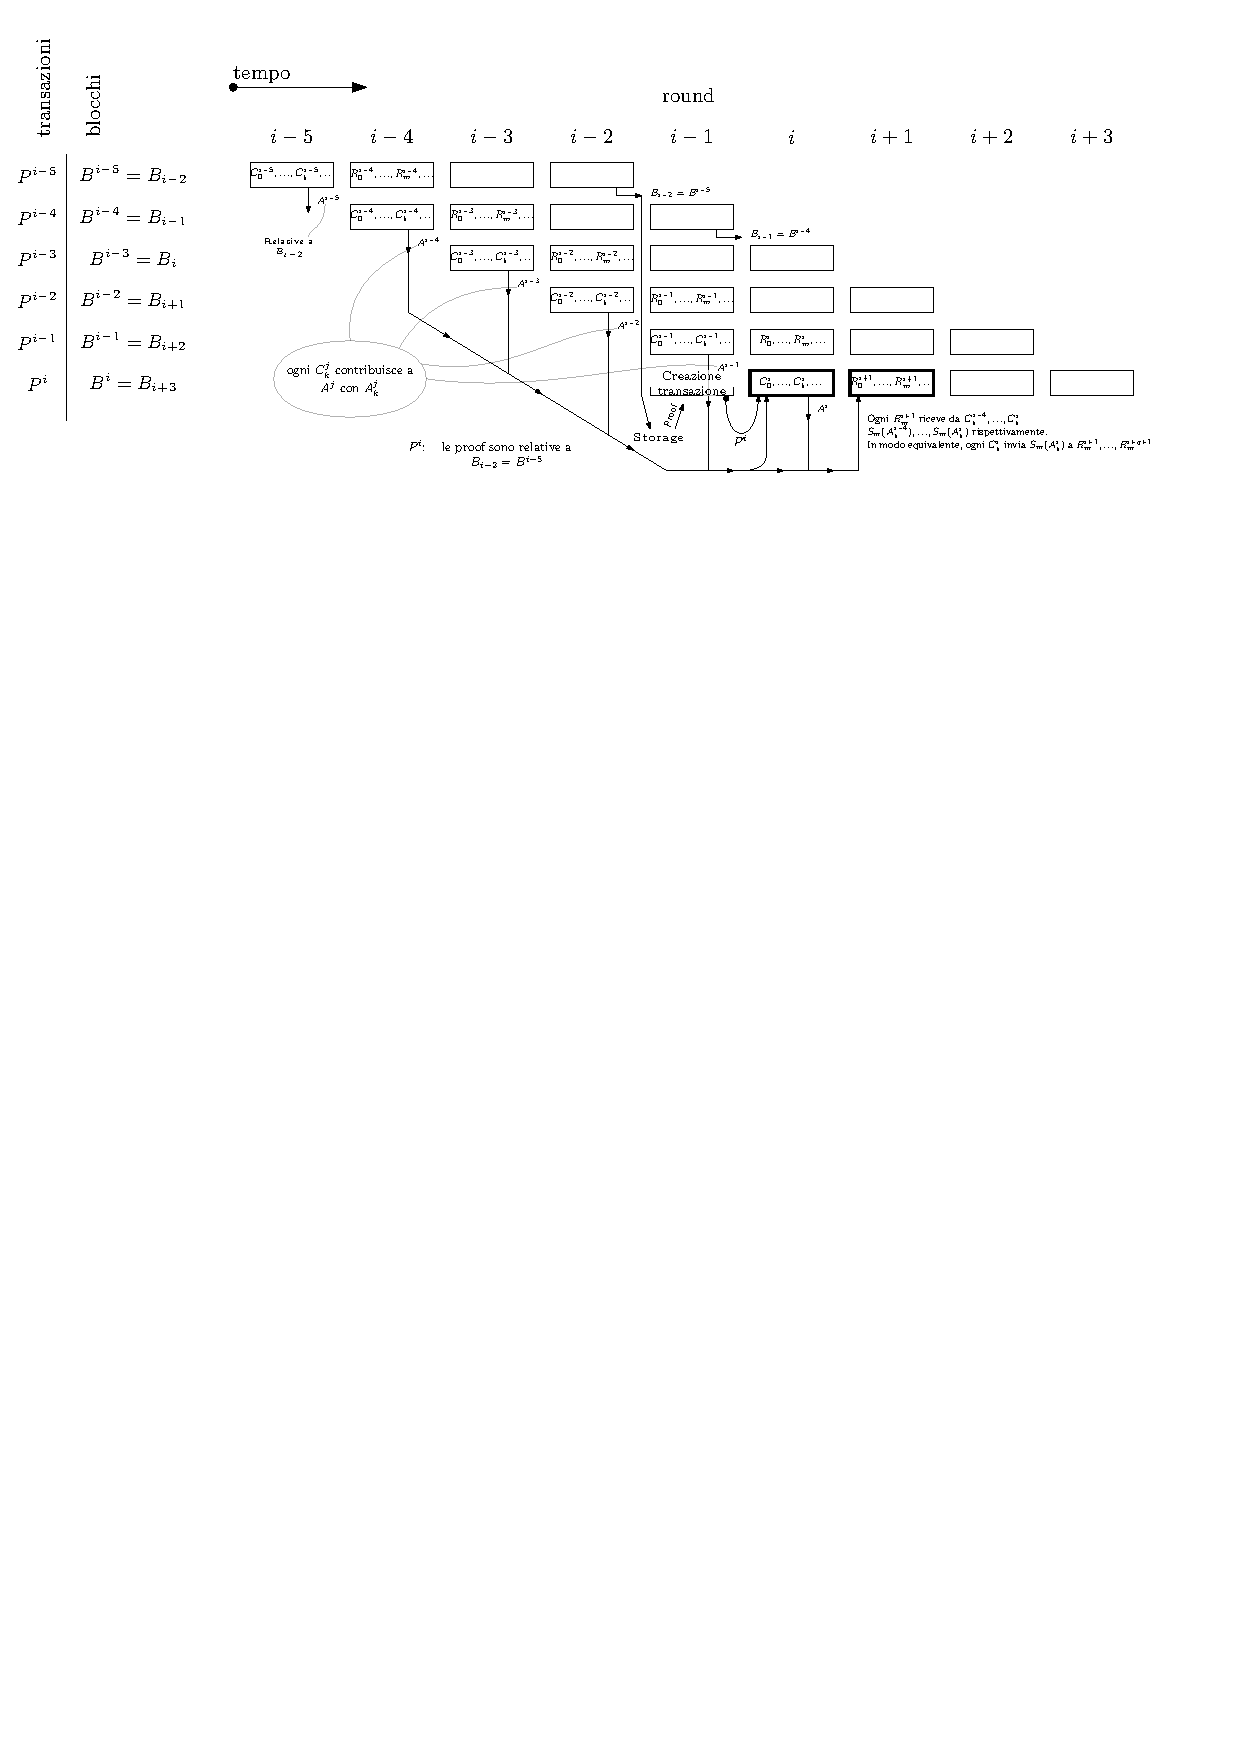
\includegraphics[scale=0.7]{img/captre/pipeline.pdf}
	\caption{Un esempio di esecuzione della pipeline con quattro stage. Nell'immagine sono sono evidenziati gli input per $C_k^i$ e $R_m^{i+1}$.}
	\label{fig:pipeline}
\end{figure}

Ogni $C_k^i$ esegue il seguente algoritmo, tramite un protocollo di consenso:

\begin{algo}{(Comportamento dei Confirmation Committee)}\label{alg:cc}
\begin{enumerate}
	\item Verifica che ogni transazione in $P(C_k^i)$ rispetti le regole sintattiche e le proof non sono scadute. Elimina le transazioni che non passano queste verifiche, generando $P'(C_k^i) \subseteq P(C_k^i)$.
	\item Seleziona una permutazione $\bar{T}$ di $P'(C_k^i)$.
	\item Sia $\tilde{T}$ la concatenazione di $A_k^{i-q}, \dots, A_k^{i-1}$. Per ogni sorgente nelle transazioni in $\bar{T}$, considera l'ultimo saldo tra i conti delle transazioni in $\tilde{T}$ e i conti forniti dalle proof delle transazioni in $\bar{T}$.
	\item Esegui le transazioni in $\bar{T}$ e verifica che il saldo risultante di ogni transazione non diventi negativo. Le transazioni che non rispettano questa regola sono scartate. Il risultato è la lista $A_k^i$ ottenuto da $\bar{T}$ dove le transazioni scartate sono omesse.	
\end{enumerate}
\end{algo}

Le transazioni in $A_k^i$ si considerano \emph{confermate} e saranno inserite nel blocco $B_i$. Per permettere ai Confirmation Committee dei round successivi di effettuare il time-updating, $C_k^i$ invia $A_k^i$ a $C_k^{i+1}, \dots, C_k^{i+q}$ ed anche ad altri comitati, come mostrato in seguito.

La lista delle transazioni confermate nel round $i$ è denotato $A^i = \bigcup_k A_k^i$, e rispetta lo stesso ordine delle transazioni in ogni $A_k^i$. Le transazioni in $A_k^i$ sono inviate anche agli storage node, anche se il blocco $B^i$ non è stato ancora creato.

La creazione del blocco $B^i = B_{i+q-1}$ richiede il calcolo dello state root-hash. Esso si ottiene dal root-hash del Merkle Tree $W$ relativo all'intero spazio dello stato, che richiede il calcolo di tutti gli hash dei nodi di $W$.
Questo è eseguito da $N_r$ comitati, denominati \emph{Root-hash Pipeline Committee}, o \emph{RPC}. Ad ogni RPC è associato una parte di $W$, denominato \emph{albero sotteso} all'RPC. Gli RPC sono disposti ad albero, denominato \emph{albero degli RPC}, come rappresentato nella Figura~\ref{fig:rpc_tree}.

\begin{figure}
	\centering
	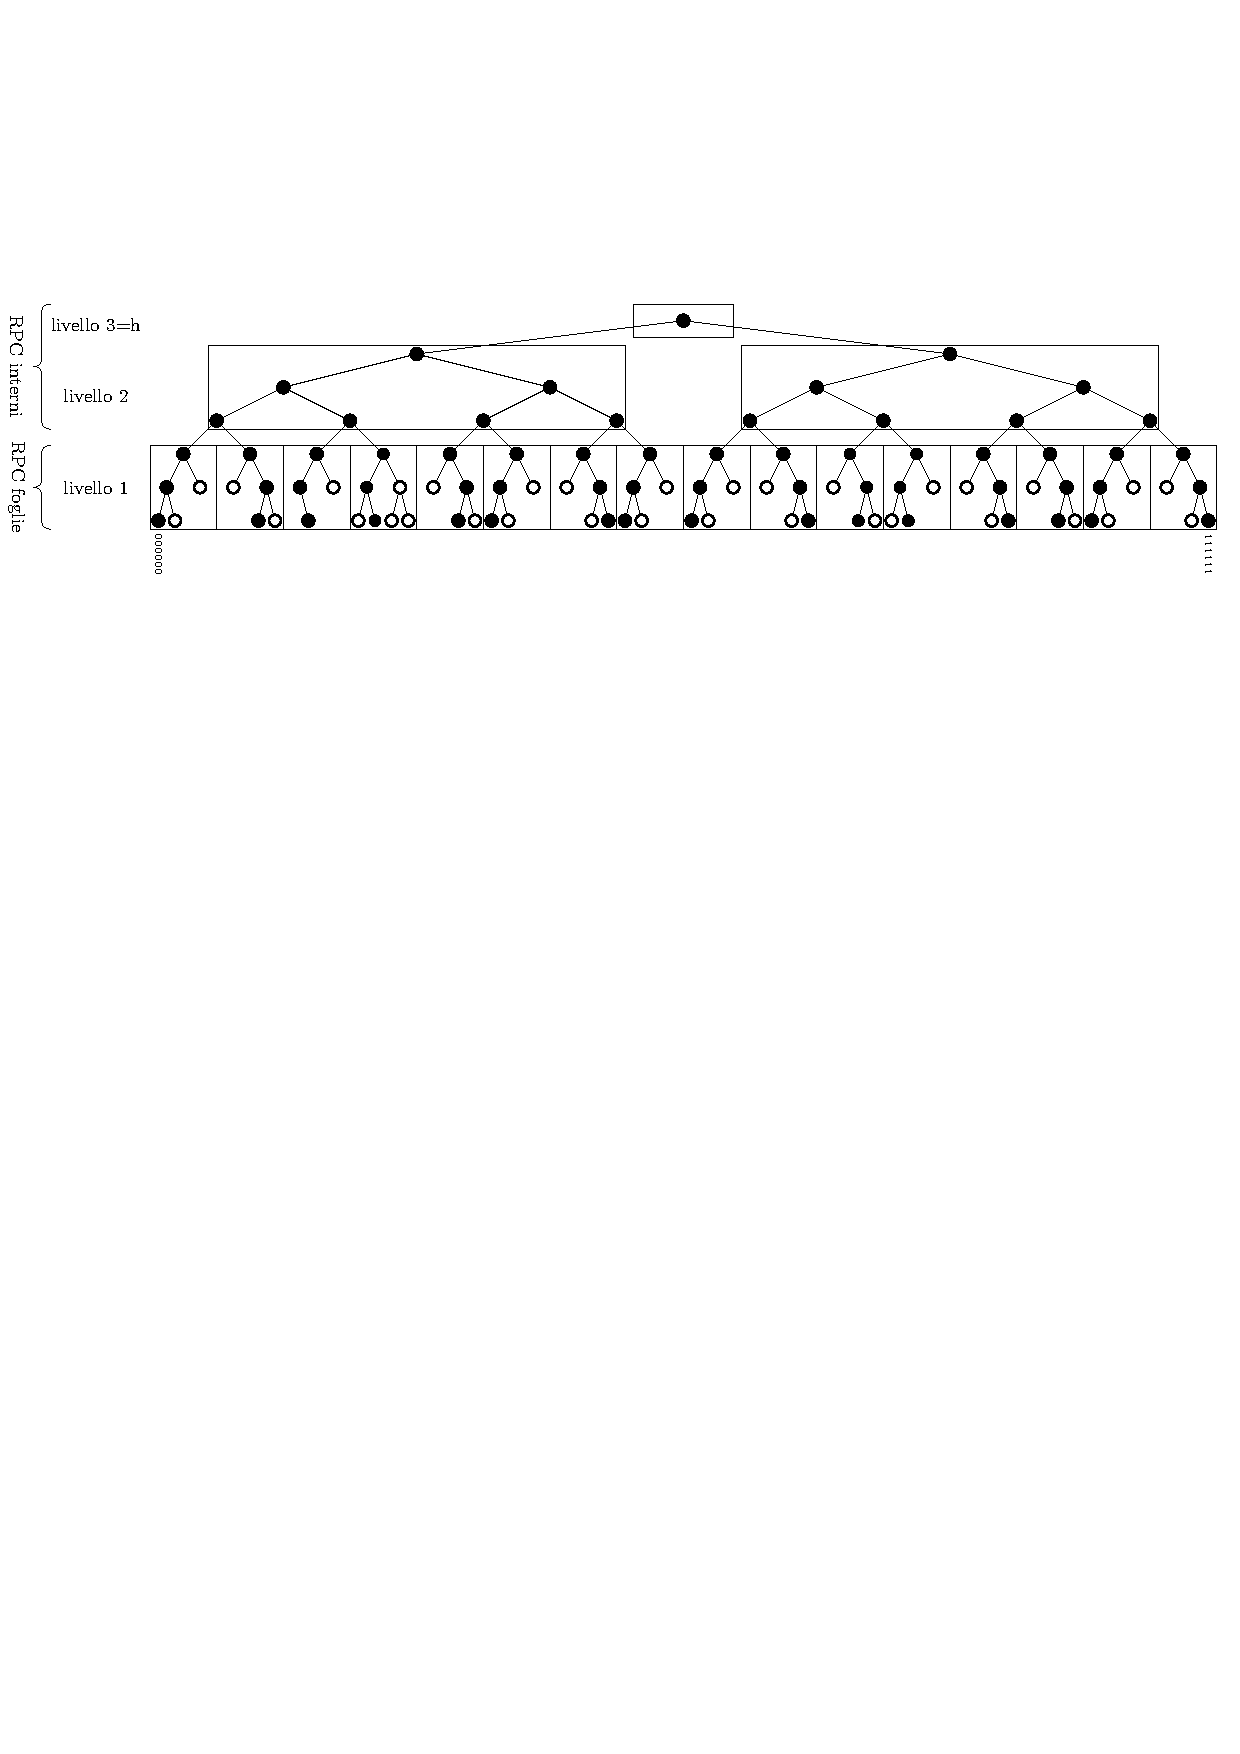
\includegraphics[scale=0.65]{img/captre/underlying_tree.pdf}
	\caption{Merkle Tree $W$ dello stato diviso tra gli RPC. I nodi bianchi sono potati.}
	\label{fig:rpc_tree}
\end{figure}

Ogni RPC ha il compito di calcolare gli hash del proprio albero sotteso durante il proprio round. Esistono due tipi di RPC: (1) gli RPC \emph{foglie}, che sono gli RPC disposti come foglie nell'albero degli RPC, e (2) gli RPC \emph{interni}, ovvero tutti gli altri. Ogni RPC foglia è responsabile di un intervallo contiguo dello spazio degli indirizzi che rappresenta le foglie di $W$. Si dice che un RPC è autorità per questo intervallo di indirizzi. Poiché solo una parte dello stato è modificato dalle nuove transazione, gli RPC foglie operano su un albero sotteso che è potato. Questo albero ha per foglie solo gli elementi di stato per cui l'RPC è autorità e che sono stati modificati dalle transazioni nel round corrente. Gli alberi sottesi degli RPC interni sono invece alberi binari completi. Gli RPC sono divisi in \emph{livelli}, numerati da $1$ ad $h$. Gli RPC foglie si trovano al livello 1, mentre a livello $h$ è presente un unico RPC, radice dell'albero degli RPC. Ad ogni livello corrisponde uno stadio della pipeline. Quindi il numero totale di stadi è $q = h+1$. Ogni albero sotteso ad un RPC ha per radice un nodo, denominato \emph{sub root-hash}. Tutti gli RPC a livello $i < h$ calcolano il proprio \emph{sub root-hash} e lo inviano ai propri genitori nell'albero degli RPC. L'RPC radice dell'albero degli RPC crea il blocco contenente lo state root-hash per il round corrente e lo invia in broadcast a tutti i nodi della rete.

Il generico RPC foglia del round $i+1$ ed autorità dell'$m$-esima porzione dello spazio degli indirizzi è denotato con $R_m^{i+1}$. Gli RPC foglie si trovano al secondo stadio della pipeline, per cui ricevono come input $A^i$, che è l'output dei Confirmation Committee del primo stadio. Tuttavia ogni RPC foglia non ha bisogno di tutte le transazioni in $A^i$, ma solo quelle che coinvolgono gli indirizzi per cui l'RPC è autorità. Se $t$ è una transazione in $A_k^i$, $C_k^i$ invia la transazione ad $R_m^{i+1}$ solo se la sorgente o la destinazione di $t$ è un indirizzo per cui $R_m^{i+1}$ è autorità. Ogni Confirmation Committee invia ogni transazione a due RPC foglie. Si denota con $S_m(A^i) \subseteq A^i$ l'insieme di transazioni che coinvolgono indirizzi che ricadono nell'intervallo $m$ e che sono ricevuti da $R_m^{i+1}$. Ogni $R_m^{i+1}$ ha il compito di calcolare il sub root-hash del proprio albero sotteso relativo al blocco $B^i$. Per questo è necessario lo stato dell'albero sotteso relativo al blocco $B^{i-1}$. Poiché le proof fornite in $S_m(A^i)$ sono relative al blocco $B_{i-2} = B^{i-q-1}$, non possono essere utilizzate da sole per il calcolo degli hash dell'albero sotteso relativo a $B^{i-1}$. Infatti gli indirizzi associati potrebbero esser stati aggiornati dalle transazioni in $A^{i-q}, \dots, A^{i-1}$ per i quali i blocchi corrispondenti non sono ancora disponibili. Quindi, ogni $R_m^{i+1}$ deve conoscere $S_m(A^{i-q}), \dots, S_m(A^{i-1})$. $R_m^{i+1}$ utilizza tutte le proof in $S_m(A^{i-q}), \dots, S_m(A^{i-1}), A^i$. $R_m^{i+1}$ per calcolare gli hash del proprio albero sotteso, come descritto nel Paragrafo~\ref{sec:bernardini}. Questo processo è chiamato \emph{time-shifting}. Per permettere agli RPC foglie dei successivi round di svolgere il proprio compito, ogni $C_k^i$ invia $S_m(A_k^i)$ a $R_m^{i+1}, \dots, R_m^{i+q+1}$.

Mentre gli RPC foglie hanno bisogno di uno stato per poter effettuare il time-shifting, gli RPC interni sono stateless. Essendo l'albero sotteso completo, hanno bisogno solamente dei sub root-hash calcolati dagli RPC figli nell'albero degli RPC, che corrispondono agli hash delle foglie dell'albero sotteso dell'RPC interno.

Ogni storage node $n$ che memorizza la potatura di $W$, le cui foglie sono gli indirizzi per cui $n$ è autorità, non può calcolarsi direttamente gli hash del proprio pADS. Quindi, durante il calcolo di $W$ relativo al blocco $B^i$, gli RPC inviano questi hash ai nodi che ne hanno bisogno. Questo può essere realizzato in maniera del tutto trasparente agli RPC, creando un canale \textit{publish/subscribe}~\cite{eugster2003many}, a cui gli storage node interessati per un sottoinsieme di nodi potati si iscrivono.

\section{Teorema di correttezza}

In questo paragrafo si dimostra formalmente la correttezza dell'architettura riportata nel Paragrafo~\ref{sec:architettura}.

\begin{lemma}{(Correttezza dell'algoritmo di conferma).}\label{lemma:cc}
L'Algoritmo 1 non restituisce mai una sequenza le cui transazioni comportano una violazione del vincolo del saldo non-negativo.
\end{lemma}

\begin{proof}
Per costruzione dello step 4 dell'Algoritmo 1.
\end{proof}


\begin{theorem}{(Correttezza).}
Sia $P^i$ un insieme di transazioni processate, nel round $i$, dai Confirmation Commitee $C_k^i$ e sia $A_k^i$ la lista delle transazioni confermate da ogni $C_k^i$. Le seguenti affermazioni sono vere.

\begin{enumerate}
	\item In ogni lista $A^i = \bigcup_k A_k^i$ tale che $A^i$ preserva l'ordine delle transazioni contenute in ogni $A_k^i$, il vincolo del saldo non-negativo è rispettato.
	\item Lo state root-hash di $B^i = B_{i+q-1}$ è il root-hash del nuovo stato ottenuto dopo l'applicazione delle transazioni in $A^i$.
	\item Gli storage node conoscono le proof degli indirizzi per cui sono autorità.
\end{enumerate}

\end{theorem}


\begin{proof}
Riguardo l'affermazione 1, per il Lemma~\ref{lemma:cc}, $A_k^i$ soddisfa il vincolo del saldo non-negativo e per ipotesi l'ordine delle transazioni in $A^i$ è preservato. Poiché per ogni $k$ gli indirizzi modificati in $A_k^i$ non sono modificati in nessun $A_j^i$ con $j \neq k$, segue l'affermazione.

Riguardo l'affermazione 2, si noti che ogni RPC foglia $R_m^{i+1}$ considera tutte le transazioni in $S_m(A^{i-q}), \dots, S_m(A^{i-1})$, che riguardano gli indirizzi per cui $R_m^{i+1}$ è responsabile, rispettando il loro ordine. Ogni $R_m^{i+1}$ può calcolare correttamente il proprio sub root-hash e passarlo al proprio RPC genitore. Infatti, se un nodo interno nell'albero sotteso è coinvolto in una transazione, $R_m^{i+1}$ riceve le proof della transazione stessa. Se un nodo interno dell'albero sotteso non è coinvolto in alcuna transazione o è potato o è la radice di un sottoalbero potato. Nel primo caso, $R_m^{i+1}$ non ne ha bisogno. Nel secondo, $R_m^{i+1}$ riceve l'hash da una delle proof presenti in $S_m(A^{i-q}), \dots, S_m(A^{i-1})$. Infine, ogni RPC interno, riceve dai propri RPC figli, gli hash delle foglie dei proprio albero sotteso, per cui il calcolo del sub root-hash è banale. Segue quindi l'affermazione.

Riguardo l'affermazione 3, si noti che gli RPC calcolano il root-hash della versione potata $W'$ di $W$, in cui le foglie di $W'$ sono tutti gli indirizzi $U$. Ogni storage node $n$ memorizza una versione potata $W_n$ di $W$, in cui le foglie di $W_n$ sono tutti gli indirizzi $U_n$ che $n$ memorizza. Poiché $U_n \subseteq U$, anche $W_n \subseteq W'$. Quindi, tutti i sub root-hash dei sottoalberi potati di $W_n$ sono conosciuti da uno degli RPC, il qualche può inviarlo ad $n$.
\end{proof}


\section{Teorema di scalabilità}

In questo paragrafo, si dimostra formalmente la scalabilità dell'architettura. Si assume, per semplicità, che i saldi modificati durante un round siano uniformemente distribuiti sullo spazio degli indirizzi.
Sia $f$ la frequenza delle transazioni che arrivano alla blockchain. Sia $\Delta$ la durata di un round. Sia $m = 2 f \Delta$ il numero di indirizzi il cui saldo viene modificato in un round, assumendo che le transazioni coinvolgano indirizzi distinti. Sia $\tilde{W}$ la versione di $W$ potata che ha solo $m$ foglie, quelle il cui saldo è modificato in un round. Esiste un livello $l$ di $\tilde{W}$ al disopra del quale $\tilde{W}$ è un albero binario completo. Più $m$ è grande, più la parte potata diventa piccola ed $l$ si avvicina alle foglie.

Sia $j$ il massimo numero di hash che un RPC può calcolare in un round. Si noti che $j$ è constante, poiché dipende dalla capacità computazionale dei nodi di un comitato. Sia $e$ il massimo numero di indirizzi il cui saldo viene modificato che un RPC foglia $R$ sia in grado di processare in un round. Ovviamente $e$ dipende da $j$ e come sono distribuiti gli indirizzi nello spazio degli indirizzi di cui $R$ è autorità. Tuttavia, per ipotesi gli indirizzi modificati sono uniformemente distribuiti, per cui $e$ è uguale per tutti gli RPC foglia. Si assume che $j$ sia grande abbastanza in modo che la radice dell'albero sotteso ad un RPC foglia sia sopra il livello $l$. Quindi, l'albero sottostante $U$ di un RPC interno $R$ è binario e completo. Sia $k$ l'altezza di $U$. Il numero di nodi di $U$ è $2^k-1$. Gli RPC figli di $R$ sono $2^{k-1}$. In ogni round, ogni RPC deve calcolare un hash per ogni nodo del proprio albero sottostante $U$. Il massimo numero di nodi in un albero sottostante ad un RPC interno è $\hat{j} = 2^{\hat{k}}-1$, dove $\hat{k}$ è il più grande numero intero tale che $\hat{j} \leq j$, o in maniera equivalente $\hat{k} = \floor*{\log_2 (j+1)}$. L'altezza massima di un di un albero sottostante ad un RPC è $\hat{k}$.

Sia $S(N, f)$ un sistema di blockchain, avente un'architettura descritta nel Paragrafo~\ref{sec:architettura}, con $N$ nodi ed un carico di frequenza $f$.

\begin{lemma}\label{lemma:rpc_count}
Sia $S(N, f)$ una blockchain, composta da $N$ nodi con un carico di frequenza $f$. Sia $e$ il massimo numero di indirizzi il cui saldo è stato modificato che un RPC foglia può processare in un round, e $\hat{j}$ il massimo numero di hash che un RPC interno può calcolare in un round. Se $S$ è ben dimensionato, il numero di RPC foglie è almeno $2^{\ceil*{\log_2 (m/e)}}$ ed il numero di RPC interni è almeno $\ceil*{\frac{2^{\ceil*{\log_2 (m/e)} - 1}}{\hat{j}}}$, in cui $m = 2 f \Delta$ e $\Delta$ è la durata di un round.
\end{lemma}

\begin{proof}
Gli RPC foglie sono almeno $\ceil*{m/e}$ e poiché sono le foglie di un albero completo, il loro numero è una potenza di 2. Quindi devono essere $2^g$ con $g = \ceil*{\log_e (m/e)}$.

Quando $m$ aumenta, il numero di risorse usate in ogni RPC foglia aumenta. Quando le risorse di un RPC foglia sono sature, il loro numero raddoppia. Immediatamente dopo un raddoppio, le loro risorse sono utilizzate a metà. Aumentando $m$, le risorse utilizzate vanno da $m$ alla massima capacità computazionale, che si ha subito prima di un raddoppio.

Si consideri l'albero composto dagli RPC interni $W_I$, la sua altezza è $g$. Poiché gli RPC foglia sono $2^g$, i nodi di $W_I$ sono $2^g -1$. Quindi il numero di RPC interni è $\ceil*{\frac{2^g-1}{\hat{j}}}$.
Da notare che sia il numeratore che il denominatore rappresentano la dimensione di un albero binario completo, con altezza $g$ e $\hat{k}$, rispettivamente. La parte intera del risultato della divisione rappresenta il numero di RPC interni con una dimensione dell'albero sottostante pari a $\hat{j}$. Il resto è la dimensione della radice dell'albero degli RPC che è più piccolo di $\hat{j}$.
\end{proof}


\begin{theorem}{(Scalabilità).}\label{th:scalability}
Sia $S(N, f)$ una blockchain well-provisioned composta da $N$ nodi ed un carico di frequenza $f$. Per ogni $\alpha > 1$ tale che $\alpha N$ è intero, la blockchain $\bar{S}(\alpha N, \alpha f)$ è well-provisioned, supponendo un carico uniformemente distribuito sullo spazio degli indirizzi.
\end{theorem}

\begin{proof}
Sia $S(N, f)$ un sistema well-provisioned immediatamente dopo un raddoppio, ovvero con gli RPC foglie al minimo delle risorse computazionali utilizzate. In $S$ e in $\bar{S}$ i comitati hanno la stessa potenza computazionale. Si vuole mostrare che $\alpha N$ nodi sono sufficienti per formare dei comitati in grado di processare in carico $\alpha f$.

Un carico di frequenza $f$, genera un numero di transazioni $f \Delta$ per round. Sia $N_C$ il numero di Confirmation Committee in $S$. Poiché, per ipotesi, $S$ è well-provisioned, ogni CC è in grado di processare $f \Delta / N_C$ transazioni per round. In $\bar{S}$ il carico è $\alpha f$, quindi, con $\alpha N_C$ CC, si ha che ogni CC in $\bar{S}$ processa lo stesso numero di transazioni che in $S$.

Si utilizzano i simboli $m$, $e$, $\hat{j}$ e $g$ con lo stesso significato di prima.
Subito dopo un raddoppio, $m/e$ è una potenza di 2, $g= \log_2 (m/e) +1$, per il Lemma~\ref{lemma:rpc_count} il numero di RPC in $S$ è $N_R = 2^g + \ceil*{2^g/\hat{j}} = 2m/e + \ceil*{2 m/ (e \hat{j})}$. Si considera ora il numero di RPC $\bar{N_R}$ necessari in $\bar{S}(\alpha N, \alpha f)$. Per $\alpha = 2^t$ con $t$ positivo ed intero, $\bar{N_R} = 2 \alpha m / e + \ceil*{2 \alpha m / (e \hat{j})}$. Poiché $\ceil{2 \alpha m/(e \hat{j}} \leq \alpha \ceil*{2 m / (e \hat{j})}$, $N_R \leq \alpha N_R$.

Quindi, l'incremento richiesto da $\bar{S}$ a partire da $S$ del numero di CC ed RPC è al massimo di un fattore $\alpha$ e $\bar{S}$ ha $\alpha N$ nodi. Quindi $\bar{S}$ è well-provisioned.
\end{proof}


\section{Comunicazione inter-committee}

Nel paragrafo precedente, nella descrizione dell'architettura, si è citata una forma di comunicazione tra comitati, o \emph{comunicazione inter-committee}, in modo che un comitato possa inviare dei dati ad un altro comitato del round successivo, oppure un nodo possa inviare la transazione candidata al CC responsabile.
Un nodo non comunica con un comitato in unicast. Questo richiederebbe infatti la conoscenza di tutte le destinazioni, che è un problema di scalabilità considerando che i membri di ogni comitato cambiano ad ogni round. Un approccio basato su multicast può essere invece una soluzione, non utilizzando però approcci tradizionali, come~\cite{fenner2016protocol}, che poco si adattano alle specifiche richieste dall'architettura.

In seguito è presentata un'analisi delle specifiche di ogni comunicazione multicast. Sia $N$ il numero dei nodi nella rete. Siano $N_C$, $N_R$, $e$, $m$, $\hat{j}$ e $q$ variabili con lo stesso significato dei precedenti paragrafi.
Sia $n$ un nodo generico nodo della rete che crea una transazione candidata. Sia $S$ la dimensione dello spazio degli indirizzi. Sia $R^i$ un Root-hash Pipeline Committee nel round $i$.

Sono stati individuati cinque flussi multicast, riportati nella Tabella~\ref{tab:multicast}.

\begin{sidewaystable}
\centering
\begin{tabular}{c|c|c|c|}
\cline{2-4}
                                                                      & \textbf{Gruppi multicast}               & \textbf{Subscriber}                                                                                                                        & \textbf{Publisher}                                  \\ \hline
\multicolumn{1}{|c|}{$n \rightarrow C_k$}                        & $N_C$                          & $\dfrac{N}{N_C + N_R}$                                                                                                            & $O(N)$                                       \\ \hline
\multicolumn{1}{|c|}{$C_k^i \rightarrow R_m^{i+1}$}                   & $\ceil*{m/e}$                  & $\dfrac{N}{N_C + N_R}$                                                                                                            & $\dfrac{N_C N}{N_C + N_R} = O(N)$          \\ \hline
\multicolumn{1}{|c|}{$R^i \rightarrow R^{i+1}$}                       & $\dfrac{\hat{j}+1}{2}^{h-i-1}$ & $\dfrac{N}{N_C + N_R}$                                                                                                            & $\dfrac{\hat{j}+1}{2}\dfrac{N}{N_C + N_R}$ \\ \hline
\multicolumn{1}{|c|}{$C_k \rightarrow DHT$}                           & S                              & \begin{tabular}[c]{@{}c@{}}ciascuno storage node\\ si iscrive ai gruppi\\ relativi agli elementi\\ di cui è autorità\end{tabular} & $\dfrac{N}{N_C + N_R}$                     \\ \hline
\multicolumn{1}{|c|}{$C_k^i \rightarrow C_k^{i+1}, \dots, C_k^{i+q}$} & $q N_C$                        & $\dfrac{N}{N_C + N_R}$                                                                                                            & $\dfrac{q N}{N_C + N_R}$                   \\ \hline
\multicolumn{1}{|c|}{$R^i \rightarrow DHT$}                           & S                              & \begin{tabular}[c]{@{}c@{}}ciascuno storage node\\ si iscrive ai gruppi\\ relativi agli elementi\\ di cui è autorità\end{tabular} & $\dfrac{N}{N_C + N_R}$                     \\ \hline
\end{tabular}
\caption{Specifiche di ogni flusso multicast.}
\label{tab:multicast}
\end{sidewaystable}


In particolare, si devono tenere in considerazione i seguenti aspetti per il multicast nella comunicazione tra comitati oppure per inviare una transazione candidata al CC autorità:

\begin{itemize}
	\item I membri di un comitato cambiano frequentemente, ad ogni round;
	\item I gruppi multicast devono essere pronti in anticipo rispetto a quando devono essere effettivamente utilizzati;
	\item I gruppi multicast sono necessari solo per un round.
\end{itemize}

Il problema della realizzazione di un multicast che rispetti queste specifiche rimane un problema aperto.

L'ultimo aspetto, una volta realizzata la comunicazione multicast, riguarda l'accettazione di un messaggio da parte di un comitato $C_{out}$ ricevuto dal comitato $C_{in}$. Infatti, $C_{in}$ potrebbe essere composto da nodi malevoli, che possono o decidere di non inviare il messaggio o di cambiarne il contenuto a proprio piacimento.
Un comitato $C_{out}$ interessato a ricevere messaggi da parte di comitato $C_{in}$, si iscrive ad un gruppo multicast come subscriber. $C_{in}$ invia i messaggi come publisher del gruppo multicast. Ogni membro del comitato $C_{in}$ invia lo stesso messaggio, che è ricevuto da ogni membro di $C_{out}$. $C_{out}$ accetta un messaggio $m$ da $C_{in}$ solo se $m$ è stato inviato da più della metà dei membri di $C_{in}$.

\section{Discussione}

In questo paragrafo si discute l'effettiva risoluzione del blockchain scalability trilemma, cercando di capire se la scalabilità limiti la decentralizzazione e/o la sicurezza, come in altri approcci presenti in letteratura.
Riguardo la \textit{decentralizzazione}, anche se ogni nodo della rete ha un ruolo diverso nella creazione del blocco, i membri ad ogni comitato sono assegnati e cambiati periodicamente in modo randomico, come in~\cite{gilad2017algorand}.
I ruoli sono quindi statisticamente omogenei. Quindi la scalabilità non impatta la decentralizzazione.

Riguardo la \textit{sicurezza}, il Teorema~\ref{th:scalability} mostra come la scalabilità non riduce la dimensione di ogni singolo comitato. Molti attacchi, come quelli presentati nel Paragrafo~\ref{attacks}, richiedono che l'attaccante controlli la maggior parte dei nodi di un comitato. Tuttavia, quando i membri di un comitato sono selezionati in modo randomico, l'attacco è molto più difficile. Inoltre, utilizzando approcci basati su Proof-of-Stake, ed in generale protocolli di consenso distribuito robusti, si evitano attacchi Sybil. Quindi la scalabilità non ha impatto sulla sicurezza.

\backmatter
\chapter{Conclusioni e Sviluppi Futuri}

La realizzazione di un'architettura che risolva il blockchain scalability trilemma è certamente un obiettivo molto ambizioso, in grado di estendere ad un uso globale tecnologie basate sulla blockchain in vari ambiti, come quello delle cripto-valute. \'E stata presentata all'interno di questo lavoro di tesi una definizione teorica di un'architettura in grado di scalare, basata su una parallelizzazione di Algorand, in cui più comitati in un round lavorano parallelamente per la creazione del prossimo blocco ed evitando la comunicazione in broadcast, che impatta fortemente la scalabilità. Si è dimostrato formalmente il suo corretto funzionamento e la scalabilità, con il teorema di correttezza e di scalabilità, rispettivamente. La scalabilità, a differenza di altre soluzione presenti in letteratura, come lo sharding, non impatta, come dimostrato, su decentralizzazione e sicurezza. La dimensione dei comitati, infatti, rimane la medesima anche a fronte di un maggior numero di transazioni. In altre parole il carico è proporzionale al numero dei nodi, mantenendo limitato il tempo di latenza per la conferma delle transazioni candidate. Quindi si può concludere che questo lavoro di tesi è il primo risultato che risolve il blockchain scalability trilemma, considerando la scalabilità di tutti gli elementi architetturali della blockchain e non solo del protocollo di consenso.

Riguardo gli sviluppi futuri, da un punto di vista teorico, è necessaria una prova formale della sicurezza sulla base di un threat model, è importante comprendere l'impatto che ha la rimozione del vincolo di sincronizzazione di tutti i nodi della rete ed il comportamento del sistema in caso di fallimento dei comitati. Inoltre, poiché è stata assunta l'esistenza di un multicast scalabile, è interessante capire come realizzare questo tipo di protocollo, fondamentale per la comunicazione tra i comitati. Infine, si potrebbe estendere il dominio di applicabilità dell'architettura, adesso focalizzato sull'ambito cripto-valute, ad un contesto più generale, introducendo gli smart contract. Da un punto di vista pratico, si può effettuare una simulazione per determinare i parametri reali del sistema.


\chapter{Ringraziamenti}
Ringrazio tutti

%bibliografia
\nocite{*}
\bibliography{bibliografia}

\end{document}